\documentclass[12pt, a4paper, notitlepage]{report}
\usepackage{indentfirst}
\usepackage{microtype}
\usepackage{listings}
\usepackage{xcolor}
\usepackage{graphicx}
\graphicspath{ {./img/} }
\usepackage{caption}
\usepackage{subcaption}
\usepackage[unicode,hidelinks]{hyperref}
\usepackage[fixlanguage]{babelbib}
\usepackage[utf8]{inputenc}
\usepackage[T1, LGR]{fontenc}
\usepackage[english, greek]{babel}

% Number subsubsections too (but don't include them in the toc)
\setcounter{secnumdepth}{3}

\newcommand{\en}[1]{\foreignlanguage{english}{#1}}
\newcommand{\gr}[1]{\foreignlanguage{greek}{#1}}
\newcommand{\blankpage}{\newpage\null\thispagestyle{empty}\newpage}
\newcommand{\osv}{\en{OSv}}
\newcommand{\viofs}{\en{virtio-fs}}
\newcommand{\qemu}{\en{QEMU}}
\newcommand{\linux}{\en{linux}}
\newcommand{\host}{\en{host}}
\newcommand{\guest}{\en{guest}}

% Provide a Greek translation for "Listing" (the listings package doesn't)
\renewcommand{\lstlistingname}{\gr{Κώδικας}}

\begin{document}

\title{
	\vspace*{-8ex}
	\begin{center}
		
\includegraphics[scale=0.4]{pyrforos.eps}
	\end{center}
	\Large{Ε}\large{ΘΝΙΚΟ}
	\Large{Μ}\large{ΕΤΣΟΒΙΟ}
	\Large{Π}\large{ΟΛΥΤΕΧΝΕΙΟ} \\
	\normalsize{Σ}\small{ΧΟΛΗ}
	\normalsize{Η}\small{ΛΕΚΤΡΟΛΟΓΩΝ}
	\normalsize{Μ}\small{ΗΧΑΝΙΚΩΝ}
	\normalsize{Κ}\small{ΑΙ}
	\normalsize{Μ}\small{ΗΧΑΝΙΚΩΝ}
	\normalsize{Υ}\small{ΠΟΛΟΓΙΣΤΩΝ} \\
	\vspace{2ex}
	\normalsize{Τ}\small{ΟΜΕΑΣ}
	\normalsize{Τ}\small{ΕΧΝΟΛΟΓΙΑΣ}
	\normalsize{Π}\small{ΛΗΡΟΦΟΡΙΚΗΣ}
	\normalsize{Κ}\small{ΑΙ}
	\normalsize{Υ}\small{ΠΟΛΟΓΙΣΤΩΝ} \\
	\vspace{14ex}
	\large\textbf{Επέκταση κοινόχρηστου με τον \host{} συστήματος αρχείων σε \en{unikernel}} \\
	\vspace{14ex}
	\largeΔΙΠΛΩΜΑΤΙΚΗ ΕΡΓΑΣΙΑ \\
	\vspace{1ex}
	\center\textbf{Φώτιος Ζαφείρης Μ. Ξενάκης}
	\vfill
	\begin{tabbing}
		\normalsize
		\textbf{Επιβλέπων}: \= Νεκτάριος Κοζύρης \\
							\> Καθηγητής Ε.Μ.Π.
	\end{tabbing}
}
\author{}	% NOTE: Just to silence the warning about missing \author
\date{
	\normalsizeΑθήνα, Οκτώβριος 2020
}
\maketitle
\thispagestyle{empty}

\blankpage

\vspace*{-8ex}
\noindent
\begin{minipage}{3.0cm}
	
\includegraphics[height=2.5cm]{pyrforos}
\end{minipage}
\begin{minipage}{12.0cm}
	Εθνικό Μετσόβιο Πολυτεχνείο \\[3pt]
	Σχολή Ηλεκτρολόγων Μηχανικών και Μηχανικών Υπολογιστών \\[3pt]
	Τομέας Τεχνολογίας Πληροφορικής και Υπολογιστών
\end{minipage}
\vspace{14ex}
\begin{center}
	\large\textbf{Επέκταση κοινόχρηστου με τον \host{} συστήματος αρχείων σε \en{unikernel}} \\
	\vspace{14ex}
	\largeΔΙΠΛΩΜΑΤΙΚΗ ΕΡΓΑΣΙΑ \\
	\vspace{1ex}
	\center\textbf{Φώτιος Ζαφείρης Μ. Ξενάκης}
\end{center}
\vfill
\begin{tabbing}
	\normalsize
	\textbf{Επιβλέπων}: \= Νεκτάριος Κοζύρης \\
						\> Καθηγητής Ε.Μ.Π.
\end{tabbing}
\vspace{4ex}
Εγκρίθηκε από την τριμελή εξεταστική επιτροπή την -TODO: ημερομηνία-.
\vspace{4ex}
\begin{center}
	\scriptsize
	\parbox[b]{0.3\textwidth} {
		\center
		........................................ \\
		Νεκτάριος Κοζύρης \\
		Καθηγητής Ε.Μ.Π.
	}
	\parbox[b]{0.3\textwidth} {
		\center
		........................................ \\
		Γεώργιος Γκούμας \\
		Επίκουρος καθηγητής Ε.Μ.Π.
	}
	\parbox[b]{0.3\textwidth} {
		\center
		........................................ \\
		Διονύσιος Πνευματικάτος \\
		Καθηγητής Ε.Μ.Π.
	}
\end{center}
\vspace{2ex}
\begin{center}
	\normalsize
	Αθήνα, Οκτώβριος 2020
\end{center}
\thispagestyle{empty}

\newpage
\vspace*{14ex}
\noindent
................................... \\
\textbf{Φώτιος Ζαφείρης Μ. Ξενάκης} \\
Διπλωματούχος Ηλεκτρολόγος Μηχανικός και Μηχανικός Υπολογιστών Ε.Μ.Π. \\
\vfill
\small
\noindent
\en{Copyright} \copyright\ Φώτιος Ζαφείρης Ξενάκης, 2020. \\
Με επιφύλαξη παντός δικαιώματος. \en{All rights reserved.}

\vspace{2ex}
\noindent
Απαγορεύεται η αντιγραφή, αποθήκευση και διανομή της παρούσας εργασίας, εξ
ολοκλήρου ή τμήματος αυτής, για εμπορικό σκοπό. Επιτρέπεται η ανατύπωση,
αποθήκευση και διανομή για σκοπό μη κερδοσκοπικό, εκπαιδευτικής ή ερευνητικής
φύσης, υπό την προϋπόθεση να αναφέρεται η πηγή προέλευσης και να διατηρείται το
παρόν μήνυμα. Ερωτήματα που αφορούν τη χρήση της εργασίας για κερδοσκοπικό σκοπό
πρέπει να απευθύνονται προς τον συγγραφέα.

\noindent
Οι απόψεις και τα συμπεράσματα που περιέχονται σε αυτό το έγγραφο εκφράζουν τον
συγγραφέα και δεν πρέπει να ερμηνευθεί ότι αντιπροσωπεύουν τις επίσημες θέσεις
του Εθνικού Μετσόβιου Πολυτεχνείου.
\thispagestyle{empty}

\newpage
\chapter*{\abstractname}
\addcontentsline{toc}{chapter}{\abstractname}

Το \en{cloud computing} είναι η κυρίαρχη προσέγγιση προς την υπολογιστική
υποδομή, βασιζόμενο στην τεχνολογία της εικονικοποίησης (\en{virtualization}).
Καθώς το \en{cloud} επεκτείνεται, καθίσταται επιτακτική η αποδοτική χρήση των
υπολογιστικών πόρων από το λογισμικό. Προς αυτό τον σκοπό, μια λύση είναι τα
\emph{\en{unikernels}}, πυρήνες λειτουργικών συστημάτων εξειδικευμένοι για να
τρέχουν μία μόνο εφαρμογή, εξοικονομώντας πόρους σε σχέση με έναν γενικού σκοπού
πυρήνα. Η αποδοτική πρόσβαση των \en{virtualized guests} στους πόρους του
\host{} συστήματος είναι μια μεγάλη πρόκληση για την εικονικοποίηση. Σε αυτόν
τον τομέα, σημαντική συνεισφορά αποτελεί το \emph{\en{virtio}}, μια προδιαγραφή
\en{paravirtualized} συσκευών για την αποδοτική χρήση των πόρων του \host{}.
Για την κοινοχρησία αρχείων ανάμεσα σε \host{} και \guest{} έχει προταθεί το
\emph{\viofs{}}, μια \en{virtio} συσκευή που προσφέρει πρόσβαση σε έναν κατάλογο
του συστήματος αρχείων του \host{} από τον \guest{}, παρέχοντας υψηλές επιδόσεις
και σημασιολογία τοπικού συστήματος αρχείων.

Αντικείμενο της παρούσας διπλωματικής εργασίας είναι η υλοποίηση και αξιολόγηση
της χρήσης του \viofs{} σε ένα \en{unikernel}. Δείχνουμε ότι ο συνδυασμός αυτών
των δύο έχει σημαντικά πλεονεκτήματα, τόσο από άποψη επιδόσεων, όσο και από
διαχειριστική άποψη στο πλαίσιο του \en{cloud}. Επίσης, τα παραπάνω γίνονται
σε πλήρη ενσωμάτωση με το έργο ανοιχτού λογισμικού του \en{unikernel} στο οποίο
βασιστήκαμε. Έτσι, το προϊόν της εργασίας αποκτά πρακτική αξία, καθώς αποτελεί
χρήσιμη συνεισφορά στο έργο, επιτυγχάνοντας έναν κεντρικό, μη τεχνικό, στόχο
της. Ταυτόχρονα, εξερευνούμε τον τρόπο λειτουργίας των έργων ανοιχτού λογισμικού
και των κοινοτήτων που σχηματίζονται γύρω τους, καθώς γινόμαστε ενεργά μέλη μίας
από αυτές.

\section*{Λέξεις κλειδιά}
\noindent
εικονικοποίηση, νέφος, σύστημα αρχείων, \en{unikernel}, \en{virtio}, \osv{},
\viofs{}, \qemu{}


\blankpage

\begin{otherlanguage}{english}
	\chapter*{\abstractname}
	\addcontentsline{toc}{chapter}{\abstractname}
	Cloud computing is the dominant approach to compute infrastructure,
	established on the technology of virtualization. As the cloud expands,
	efficient utilization of its compute resources by software becomes
	imperative. One solution towards that are \emph{unikernels}, operating
	system kernels specialized to run a single application, sparing resources
	compared to a general-purpose kernel. Efficient access from virtualized
	guests to the underlying host's resources is a substantial challenge in
	virtualization. In this aspect, \emph{virtio} has been a significant
	contribution, as a specification of paravirtual devices enabling efficient
	usage of the host's resources. For host-guest file sharing, \emph{\viofs{}}
	has been proposed, as a virtio device offering guest access to a file system
	directory on the host, providing high performance and local file system
	semantics.

	This thesis is concerned with the implementation and evaluation of \viofs{}
	in the context of the \osv unikernel. We demonstrate that combining the two
	offers great benefits, both with regard to performance achieved, which
	is comparable to local file systems, and the operational aspect in a cloud
	context. Moreover, the above are carried out fully within the open-source
	project behind the unikernel we based our work on. This way, the resulting
	product gains practical value, being a useful contribution to the project,
	thus achieving a pivotal, non-technical goal. Furthermore, we explore how
	open-source software projects and the communities around them work, as we
	become active members of one.

	\section*{Keywords}
	\noindent
	virtualization, cloud, file system, unikernel, virtio, \osv{}, \viofs{},
	\qemu{}
\end{otherlanguage}


\blankpage

\chapter*{Ευχαριστίες}
\addcontentsline{toc}{chapter}{Ευχαριστίες}
Για την παρούσα εργασία, που σηματοδοτεί την ολοκλήρωση μίας πορείας ετών, θα
ήθελα να ευχαριστήσω τα μέλη του εργαστηρίου υπολογιστικών συστημάτων, υπό την
αιγίδα του οποίου πραγματοποιήθηκε. Πιο πολύ όμως θα ήθελα να τους ευχαριστήσω,
όπως και άλλα μέλη της σχολής ΗΜΜΥ, για τη διδασκαλία, το γνήσιο ενδιαφέρον και
την καλλιέργεια της κουλτούρας του μηχανικού που μου προσέφεραν.

Επίσης, οφείλω ένα μεγάλο ευχαριστώ στους ανθρώπους των κοινοτήτων του \osv{}
και του \viofs{} για την υποστήριξη, τις συμβουλές και το χρόνο τους, αλλά
κυρίως για την ανοικτότητα, το ήθος και το έργο τους, που ενέπνευσαν αυτή τη
συμβολή.

Τέλος, αυτοί για τους οποίους είμαι περισσότερο ευγνώμων είναι η οικογένεια και
οι φίλοι μου, που πάντα βρίσκονται στο πλευρό μου, με ανέχονται και με στηρίζουν
και χωρίς τους οποίους τίποτα δεν θα μπορούσε να επιτευχθεί.


\blankpage

\tableofcontents
\addcontentsline{toc}{chapter}{\contentsname}

\listoffigures
\addcontentsline{toc}{chapter}{\listfigurename}

\listoftables
\addcontentsline{toc}{chapter}{\listtablename}

\chapter{Εισαγωγή}

\section{Κίνητρο}

\subsection{Γιατί \en{unikernel}}
Η τελευταία δεκαετία έχει χαρακτηριστεί από την κυριαρχία του μοντέλου του
υπολογιστικού νέφους (\en{cloud computing}) στην υπολογιστική υποδομή. Αυτό έχει
εξελιχθεί σε θεμέλιο λίθο σε πολλά πεδία εφαρμογών, κάνοντας πρακτικές
αρχιτεκτονικές που μέχρι πρότινος ήταν αδύνατες, για ένα ολοένα αυξανόμενο
πλήθος χρηστών. Επίσης, η ευρύτατη υιοθέτηση του έχει οδηγήσει σε διαχείριση
υπολογιστικών πόρων πρωτοφανούς κλίμακας. Η τεχνολογία που καθιστά δυνατό το
\en{cloud} στην παρούσα του μορφή είναι αυτή της εικονικοποίησης: της κατά
βούληση ``σμίλευσης'' πολλαπλών εικονικών μηχανών (\en{guests}) από ένα φυσικό
σύστημα (\host{}).

Παρά τις μεγάλες αλλαγές που έχει φέρει η έλευση του \en{cloud}, τα παραδοσιακά
κομμάτια της στοίβας λογισμικού, με κύριο εκπρόσωπο το λειτουργικό σύστημα,
έχουν επηρεαστεί ελάχιστα από αυτήν. Έτσι, σε αυτή την πλευρά κυριαρχούν τα
λειτουργικά συστήματα γενικού σκοπού όπως το \linux{}, με σχεδιαστικές επιλογές
και κληρονομιά δεκαετιών. Το γεγονός αυτό είναι αδιαμφισβήτητα ενδεικτικό της
υψηλής δυσκολίας που έχει η υλοποίηση τους, αλλά και της αξίας που έχουν τα
παρόντα συστήματα, κατόπιν συσσώρευσης μακράς αλυσίδας βελτιώσεων.

Ένας συνδυασμός παραγόντων όμως καθιστά πλέον εμφανές ότι τα γενικού σκοπού
λειτουργικά συστήματα δεν είναι η βέλτιστη λύση για τις ανάγκες των σύγχρονων
εφαρμογών. Σε αυτούς τους παράγοντες συγκαταλέγεται η μετάβαση από φυσικά σε
εικονικά μηχανήματα με την ακύρωση της υπόθεσης της αποκλειστικής χρήσης των
πόρων που αυτή συνεπάγεται. Επίσης, το ταχύ κλείσιμο του άλλοτε χάσματος ανάμεσα
στις επιδόσεις \en{I/O} και επεξεργασίας, που καθιστά σχεδόν απαγορευτική την
εμπλοκή του λειτουργικού συστήματος στο μονοπάτι δεδομένων (\en{data path}) μίας
εφαρμογής που απαιτεί ύψιστες επιδόσεις, εξ' ου και η δημοφιλία των \cite{dpdk,
spdk}. Τέλος, η προαναφερθείσα κλίμακα των υποδομών, που ενισχύει την ανάγκη για
βελτιστοποίηση της αποδοτικότητας, καθώς η υποβέλτιστη λειτουργία έχει μεγάλο
κόστος.

Τα \en{unikernels} είναι μία αξιόλογη πρόταση για αντικατάσταση των συμβατικών
λειτουργικών συστημάτων στους \en{guests}, όταν αυτά χρησιμοποιούνται για την
εκτέλεση μίας μόνο εφαρμογής. Προκύπτουν από τη συγχώνευση μίας εφαρμογής μαζί
με όσα υποστηρικτικά στοιχεία αυτή χρειάζεται (που τυπικά παρέχονται από το
λειτουργικό σύστημα), υπό τη μορφή βιβλιοθηκών, σε έναν κοινό χώρο διευθύνσεων.
Οι παραγόμενες εκτελέσιμες εικόνες εκτελούνται ως εικονικές μηχανές
επιτυγχάνοντας υψηλότερη αποδοτικότητα, αφού έχουν μικρότερο μέγεθος (οπότε
ταχύτερη μεταφορά και εκκίνηση \cite{jitsu} και χαμηλότερες απαιτήσεις
αποθηκευτικού χώρου), χαμηλότερες απαιτήσεις μνήμης και πιο αποδοτικές
λειτουργίες συστήματος λόγω πχ έλλειψης \en{mode switches} και απλουστευμένου
μοντέλου ασφάλειας.

\subsection{Γιατί κοινό σύστημα αρχείων και \viofs{}}
Τυπικά, τα συστήματα αρχείων είναι τοπικά, υλοποιημένα με συσκευές \en{block},
στο πλαίσιο του πυρήνα ενός λειτουργικού συστήματος. Υπάρχουν όμως περιπτώσεις
οι οποίες ωφελούνται από την κοινή χρήση του ίδιο συστήματος αρχείων από
περισσότερα συστήματα. Μία τέτοια περίπτωση είναι αυτή της εικονικοποίησης, όπου
\host{} και \guest{} μοιράζονται ένα σύστημα αρχείων (το οποίο συνήθως
προϋπάρχει στον \host{}). Ένα παράδειγμα όπου είναι σαφής η χρησιμότητα του
παραπάνω είναι στην εκκίνηση εικονικών μηχανών οι οποίες (ανα)διαμορφώνονται από
τον \host{}, ενώ ένα άλλο είναι η εκτέλεση βραχύβιων εικονικών μηχανών που
διαβάζουν δεδομένα εισόδου ή διαμόρφωσης και γράφουν δεδομένα εξόδου σε ένα
κοινόχρηστο σύστημα αρχείων.

Το \viofs{} είναι μια πρόσφατη προσπάθεια στο πεδίο των κοινόχρηστων συστημάτων
αρχείων, η πρώτη χτισμένη από την αρχή με αποκλειστικό στόχο τα περιβάλλοντα
εικονικοποίησης. Αυτή η εξειδίκευση του επιτρέπει να μην έχει καμία εξάρτηση
από δικτυακά πρωτόκολλα ή (εικονική) δικτυακή υποδομή, οδηγώντας αφενός σε
χαμηλότερες απαιτήσεις από τον \guest{} για τη χρήση του, αφετέρου σε καλύτερες
επιδόσεις και προσφορά σημασιολογίας τοπικού συστήματος αρχείων
\cite{virtiofs-website}. Σημαντικό ρόλο στην επίτευξη των προηγούμενων παίζει η
χρήση ενός χώρου κοινής μνήμης μεταξύ \host{} και \guest{} όπου απεικονίζονται
τα περιεχόμενα των αρχείων, το λεγόμενο \en{DAX (Direct Access) window}. Τα
παραπάνω το καθιστούν ιδανικό για χρήση σε ``\en{lightweight}'' \en{guests},
συμπεριλαμβανομένων των \en{unikernels}.

\section{Στόχοι}
Αυτή η εργασία έχει σκοπό την εξερεύνηση των δυνατοτήτων που προσφέρει το
\viofs{} σε ένα \en{unikernel}. Συγκεκριμένα, επιλέγουμε το \osv{} και
επεκτείνουμε την ήδη υπάρχουσα, στοιχειώδη υλοποίηση του για το \viofs{},
προσθέτοντας μεταξύ άλλων (\en{read-only}) υποστήριξη για το \en{DAX window}
καθώς και δυνατότητα εκκίνησης (\en{boot}) από ένα \viofs{} σύστημα αρχείων.
Έτσι καθίσταται πρακτική η χρήση του σε πολλές περιπτώσεις. Επίσης, αξιολογούμε
τις επιδόσεις της υλοποίησης μας σε σύγκριση με πλήθος άλλων συστημάτων αρχείων,
σε ένα εύρος αντιπροσωπευτικών σεναρίων.

Η εργασία όμως έχει και μη τεχνικούς στόχους που έχουν να κάνουν με το
μοντέλο του ελεύθερου λογισμικού / λογισμικού ανοιχτού κώδικα. Μιας και αμφότερα
τα έργα που εμπλέκονται (\osv{} και \viofs{}) είναι έργα ελεύθερου λογισμικού,
θεωρούμε ευκαιρία αλλά και υποχρέωση όλες οι επεκτάσεις μας στο \osv{} να
προσφερθούν για συμπερίληψη σε αυτό. Με αυτόν τον τρόπο και άλλοι χρήστες
του έργου μπορεί να επωφεληθούν από την εργασία μας, η οποία αποκτά αξία πέραν
της ακαδημαϊκής, ενώ, τέλος, οι κοινότητες των έργων αποκτούν ένα νέο, ενεργό
μέλος.

\section{Σχετική δουλειά}
Στα χρόνια από την ανακοίνωση του \en{MirageOS} \cite{mirageos} έχουν κάνει την
εμφάνιση τους πληθώρα \en{unikernel frameworks}, σχηματίζοντας ένα πολυποίκιλο
σύνολο. Μερικά, εκτός του \osv{}, είναι τα \en{RumpRun} \cite{rumprun},
\en{IncludeOS} \cite{includeos}, \en{HermitCore} \cite{hermitcore} και
\en{HermiTux} \cite{hermitux}, \en{ukl} \cite{ukl}, \en{Toro} \cite{toro} και
\en{Nanos} \cite{nanos}.

Η κυριότερη, προϋπάρχουσα εναλλακτική του \viofs{} είναι το \en{VirtFS}
\cite{virtfs} που βασίζεται στο δικτυακό πρωτόκολλο \en{9P} \cite{9p}. Το
\viofs{} είναι ακόμα ένα νεό έργο, υπό ενεργή ανάπτυξη, γι' αυτό και είναι
διαθέσιμες σχετικά λίγες υλοποιήσεις του. Από τη μεριά του \host{}, πέρα από την
κύρια υλοποίηση του στο \qemu{} \cite{virtiofs:qemu}, υπάρχει πλήρης υλοποίηση
του \viofs{} στον \en{cloud-hypervisor} \cite{cloud-hypervisor}, μία εναλλακτική
υλοποίηση του \en{virtiofsd} ονόματι \en{memfsd} από την κοινότητα των \en{nabla
containers} \cite{memfsd} καθώς και μία υλοποίηση στο \en{firecracker}
\cite{firecracker}η οποία έχει απορριφθεί προς το παρόν. Από τη μεριά του
\guest{}, πέρα από την κύρια υλοποίηση του στο \linux{} \cite{virtiofs:linux},
υπάρχει υλοποίηση στο \en{Toro} (ένα ακόμα \en{unikernel}, γραμμένο σε
\en{Pascal}) \cite{toro}, όπως και για \en{Windows} \cite{virtio-windows}.

\section{Οργάνωση του παρόντος}
Στο δεύτερο κεφάλαιο δίνεται μία πλήρης περιγραφή όλου του τεχνικού υποβάθρου
της εργασίας, από τις περιπτώσεις χρήσης του \en{cloud} έως και τις τεχνολογίες
με χρήση των οποίων υλοποιείται το \viofs{}. Το κεφάλαιο τρία αναλύει τη
διαδικασία και τα χαρακτηριστικά της υλοποίησης των επεκτάσεων μας στο \osv{}.
Το τέταρτο κεφάλαιο καταπιάνεται με την αξιολόγηση της τελευταίας, περιγράφοντας
τη μεθοδολογία που ακολουθήθηκε και εξετάζοντας τα αποτελέσματα, ενώ το πέμπτο
και τελευταίο κεφάλαιο περιέχει μία σύντομη ανασκόπηση και κατευθύνσεις για
περαιτέρω δουλειά στο μέλλον.

\chapter{Υπόβαθρο}

\section{Υπολογιστικό νέφος}
Το υπολογιστικό νέφος (\en{cloud computing}) είναι ένα μοντέλο παροχής
υπολογιστικών πόρων ως υπηρεσίας το οποίο εδραιώνεται πλέον ως κυρίαρχο.
Βασίζεται στην παροχή συγκεντρωμένων, κοινόχρηστων υπολογιστικών πόρων κατ'
απαίτηση (\en{on demand}), μέσω δικτύου. Αυτοί οι φυσικοί πόροι
ανήκουν και διαχειρίζονται από έναν πάροχο υπηρεσιών νέφους (\en{cloud service
provider}) και γίνονται διαθέσιμοι εξ' αποστάσεως σε χρήστες - πελάτες, οι
οποίοι έτσι επιτυγχάνουν χαμηλότερο αρχικό κόστος για υπολογιστική υποδομή,
ευελιξία, κλιμακωσιμότητα, συντομότερο χρόνο \en{deployment} και απλοποιημένη
διαχείριση \cite{wiki:cloud}.

Διακρίνονται τρία βασικά μοντέλα υπηρεσιών \en{cloud} μέσω των οποίων παρέχεται
πρόσβαση στην υποκείμενη υπολογιστική υποδομή, όπως φαίνεται και στο σχήμα
\ref{fig:cloud} \cite{nist-cloud}:
\begin{description}
    \item[\en{Infrastructure-as-a-Service (IaaS)}] όπου γίνονται διαθέσιμοι
        υπολογιστικοί πόροι επεξεργασίας (\en{compute}), αποθήκευσης
        (\en{storage}) και δικτύωσης, όπως εικονικές μηχανές (\en{virtual
        machines}), μονάδες αποθήκευσης, εικονικά δίκτυα και εξισορροπητές
        φόρτου (\en{load balancers}). Αυτό είναι το μοντέλο που προσφέρει το
        μικρότερο επίπεδο αφαίρεσης (\en{abstraction}) παράλληλα με την
        μεγαλύτερη ευελιξία στους χρήστες.
    \item[\en{Platform-as-a-Service (PaaS)}] στο οποίο παρέχεται η δυνατότητα
        στους χρήστες να αναπτύξουν τις εφαρμογές τους λαμβάνοντας ως δεδομένο
        το ``περιβάλλον'' στο οποίο αυτές θα εκτελεστούν. Ουσιαστικά, σε αυτό το
        μοντέλο τους παρέχεται μία υπηρεσία υψηλότερου επιπέδου με την έννοια
        ότι δεν έχουν την ευθύνη της διαχείρισης συστατικών όπως το λειτουργικό
        σύστημα και το σύστημα χρόνου εκτέλεσης (\en{runtime system}), αφήνοντας
        τους να επικεντρωθούν στην εφαρμογή.
    \item[\en{Software-as-a-Service (SaaS)}] όπου πρόκειται για το πιο υψηλό
        επίπεδο αφαίρεσης από την υπολογιστική υποδομή. Σε αυτό δίνεται
        πρόσβαση στους χρήστες σε συγκεκριμένες εφαρμογές, οι οποίες
        διαχειρίζονται πλήρως από τον πάροχο, από την υπολογιστική υποδομή μέχρι
        και την έκδοση και διαμόρφωση της ίδιας της εφαρμογής. Παραδείγματα
        αποτελούν υπηρεσίες ηλεκτρονικής αλληλογραφίας (\en{email}), διαχείρισης
        έργων (\en{project management}) και εφαρμογών γραφείου όπως επεξεργασίας
        εγγράφων και υπολογιστικών φύλλων (\en{spreadsheets}).
\end{description}

\begin{figure}
    \centering
    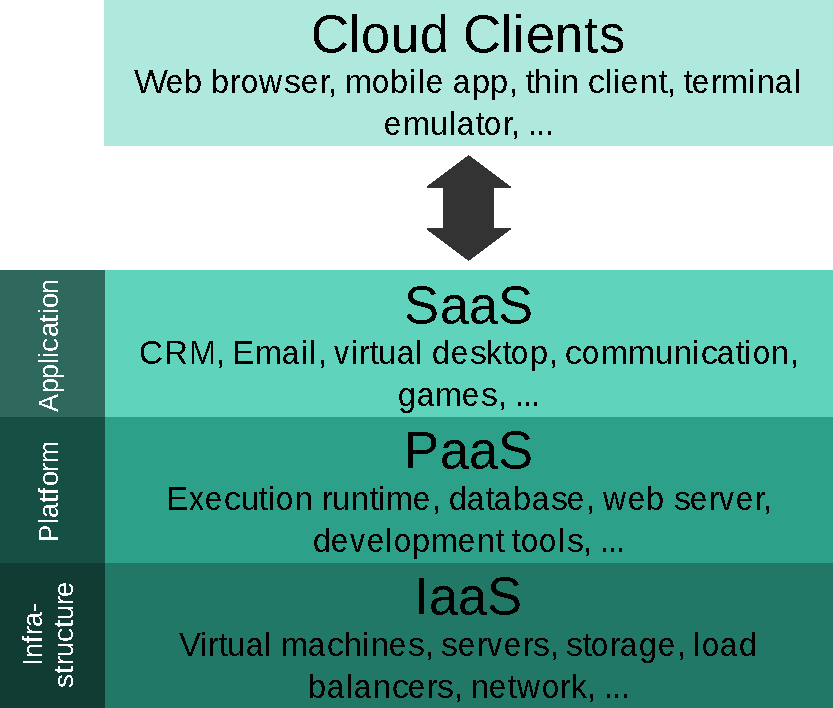
\includegraphics[scale=0.8]{cloud-layers}
    \caption[Μοντέλα παροχής υπηρεσιών \en{cloud}]{Μοντέλα παροχής υπηρεσιών
        \en{cloud}. Πηγή
        \en{\href{https://commons.wikimedia.org/wiki/File:Cloud_computing_layers.svg}{Wikimedia Commons}}.}
    \label{fig:cloud}
\end{figure}

Ένα μοντέλο που έχει κάνει την εμφάνιση του πιο πρόσφατα και έχει ελκύσει
πολλούς χρήστες είναι το λεγόμενο \en{serverless} ή \en{Function-as-a-Service
(FaaS)}. Αυτό ταιριάζει με το \en{PaaS} (θα μπορούσε να θεωρηθεί κομμάτι ή
εξέλιξη του), καθώς όπως υποδηλώνει το όνομα του, αφαιρεί εξ' ολοκλήρου την
ευθύνη του \en{server} από τους χρήστες της υπηρεσίας. Τα τεχνικά χαρακτηριστικά
στα οποία δίνεται έμφαση είναι η αυτόματη κλιμακωσιμότητα από το μηδέν μέχρι και
πολύ μεγάλη κλίμακα καθώς και η άμεση απόκριση σε διακυμάνσεις του φόρτου,
μιας και η εκκίνηση και ο τερματισμός στιγμιοτύπων της εφαρμογής είναι πολύ
γρήγορες διαδικασίες \cite{cloudflare-serverless}. Ένα μειονέκτημα του
\en{serverless} είναι ότι κάποιες μόνο εφαρμογές ταιριάζουν σε αυτό το μοντέλο,
οπότε είναι δυνατό να επωφεληθούν από τα παραπάνω \cite{serverless,
spec-serverless}.

\section{Εικονικοποίηση}
Η τεχνολογία που βρίσκεται κατά κύριο λόγο πίσω από το \en{cloud} είναι αυτή της
εικονικοποίησης (\en{virtualization}). Με αυτήν προστίθεται ένα επίπεδο
αφαίρεσης πάνω από την φυσική υπολογιστική υποδομή, αφού επιτρέπει την
απεικόνιση ενός (συνήθως μεγάλου) φυσικού μηχανήματος (\en{host}) σε
περισσότερα, μικρότερα εικονικά μηχανήματα (\en{virtual machines -- guests}), τα
οποία δημιουργούνται, τροποποιούνται, μεταφέρονται και καταργούνται δυναμικά,
μέσω λογισμικού, θέτοντας τα θεμέλια για τις σύγχρονες υπηρεσίες \en{cloud}
\cite{wiki:hw-virtualization}.

Ως προς τις απαιτήσεις από το λογισμικό που εκτελείται ως \guest{} διακρίνονται
δύο περιπτώσεις:
\begin{description}
    \item[Πλήρης εικονικοποίηση (\en{full virtualization})] όπου ο \guest{} δεν
        αντιλαμβάνεται ότι εκτελείται από ένα εικονικό μηχάνημα. Έτσι, δεν
        απαιτούνται αλλαγές ώστε λογισμικό που έχει δημιουργηθεί για φυσικά
        μηχανήματα να εκτελεστεί σε εικονικά.
    \item[\en{Paravirtualization}] όπου ο \guest{} τροποποιείται ειδικά για την
        εκτέλεση του στο \en{virtual machine}.
\end{description}
Η εικονικοποίηση ήταν παρούσα για δεκαετίες πριν την έλευση του \en{cloud}.
Καθοριστικό σημείο για την υλοποίηση αυτού ήταν η προσθήκη υποστήριξης υλικού
για την εικονικοποίηση στην αρχιτεκτονική \en{x86}, που οδήγησε στην αποδοτική
χρήση της, χωρίς υψηλές απαιτήσεις από το λογισμικό \cite{virtualization-x86}.
Μέχρι εκείνο το σημείο η εικονικοποίηση σε αυτή τη δημοφιλή αρχιτεκτονική
βασιζόταν σε τεχνικές \en{paravirtualization}.

Την ευθύνη για την υλοποίηση της εικονικοποίησης έχει ο λεγόμενος
\en{hypervisor} ή \en{virtual machine monitor (VMM)}. Αυτός είναι συνήθως
λογισμικό, εκτελούμενο στον \host{} με αυξημένα δικαιώματα (\en{privileges}).
Το έργο του περιλαμβάνει την εκκίνηση των εικονικών μηχανών και την
εξομοίωση των ενεργειών που δεν επιτρέπονται σε αυτές, με κυριότερη την
αλληλεπίδραση με τις περιφερειακές συσκευές του συστήματος. Το δεύτερο τυπικά
υλοποιείται με την τεχνική \en{trap and emulate}, όπου συγκεκριμένες εντολές
κατά την εκτέλεση της εικονικής μηχανής προκαλούν \en{traps} στον επεξεργαστή
με συνέπεια τη μεταφορά στον κώδικα του \en{hypervisor}. Εκείνος αναλαμβάνει
να ελέγξει και να εκτελέσει την ενέργεια που επιχείρησε ο \guest{},
επιστρέφοντας κατόπιν τον έλεγχο στο σημείο όπου είχε σταματήσει αυτός. Ο
μηχανισμός ετούτος δίνει στον \en{hypervisor} πλήρη έλεγχο στο μοντέλο
(εικονικών) συσκευών (\en{device model}) του \en{virtual machine}
\cite{wiki:hypervisor}.

Οι \en{hypervisors} διακρίνονται σε δύο πρωταρχικές κατηγορίες (σχήμα
\ref{fig:hypervisors}) \cite{popek74}:
\begin{description}
    \item[Τύπου 1] οι οποίοι εκτελούνται απευθείας πάνω από το φυσικό μηχάνημα,
        αναλαμβάνοντας εξ' ολοκλήρου τη διαχείριση του, πέρα από τη διαχείριση
        των εικονικών μηχανών. Τυπικά αυτοί οι \en{hypervisors} εξαρτώνται από
        έναν \guest{} ειδικού σκοπού, ο οποίος έχει αυξημένα προνόμια σε
        σχέση με τους υπόλοιπους, ώστε να διαχειρίζεται τις συσκευές του
        μηχανήματος, διαθέτοντας τους κατάλληλους οδηγούς (\en{drivers}). Ο πιο
        γνωστός εκπρόσωπος ελεύθερου λογισμικού αυτής της κατηγορίας είναι ο
        \en{Xen} \cite{xen}.
    \item[Τύπου 2] οι οποίοι εκτελούνται ως μέρος ενός τυπικού λειτουργικού
        συστήματος, αναλαμβάνοντας μόνο την εκκίνηση και παρακολούθηση των
        εικονικών μηχανών, ενώ η διαχείριση του \host{} γίνεται από το
        λειτουργικό, ως συνήθως. Σε αυτή την κατηγορία ο κάθε \guest{} συχνά
        είναι απλά μία διεργασία από την σκοπιά του \host{}. Το πιο γνωστό
        παράδειγμα ελεύθερου λογισμικού που ανήκει σε αυτή την κατηγορία είναι
        το \qemu{} \cite{qemu} (τυπικά σε συνδυασμό με το \en{KVM} \cite{kvm},
        το οποίο παρέχει επιτάχυνση υλικού).
\end{description}

\begin{figure}
    \centering
    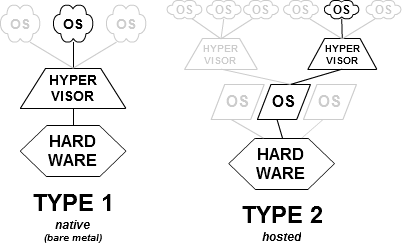
\includegraphics[scale=0.7]{hypervisors}
    \caption[Τύποι \en{hypervisors}]{Τύποι \en{hypervisors}. Πηγή
        \en{\href{https://commons.wikimedia.org/wiki/File:Hyperviseur.png}{Wikimedia Commons}}.}
    \label{fig:hypervisors}
\end{figure}

\section{\en{Unikernels}}
Στην πλέον συνήθη περίπτωση χρήσης της εικονικοποίησης, μπορούμε να θεωρήσουμε
το λογισμικό που υποστηρίζει την εκτέλεση μίας εφαρμογής ως εξής (σχηματικά στο
\ref{fig:components-vm}):
\begin{itemize}
    \item Στον \host{} (\en{kernel space}) εκτελείται ένα γενικού σκοπού
        λειτουργικό σύστημα που έχει απευθείας πρόσβαση στους πόρους του φυσικού
        μηχανήματος και είναι υπεύθυνο γι' αυτούς.
    \item Στον \host{} (τυπικά \en{user space}) εκτελείται επίσης ο
        \en{hypervisor}, αναλαμβάνοντας τη διαχείριση των εικονικών μηχανών που
        αντιστοιχούν στο σύστημα.
    \item Στον \guest{} (\en{kernel space}) εκτελείται και πάλι ένα στιγμιότυπο
        λειτουργικού συστήματος γενικού σκοπού. Αυτό έχει την ευθύνη των πόρων
        του εικονικού μηχανήματος, όπως έχουν ανατεθεί από τον \en{hypervisor}.
    \item Στον \guest{} (\en{user space}) εκτελείται η εφαρμογή, συχνά μαζί με
        συστατικά όπως βιβλιοθήκες τρίτων και συστήματα χρόνου εκτέλεσης
        (\en{runtime systems}).
\end{itemize}
Η στοίβα αυτή λογισμικού περιέχει διπλότυπα και υψηλή πολυπλοκότητα, δύο
στοιχεία τυπικά υπαίτια για προβλήματα όπως η υποβέλτιστη χρησιμοποίηση των
πόρων και οι μειωμένες επιδόσεις λόγω \en{overheads} (πχ \en{mode switches}) στη
συνολική λειτουργία του συστήματος, αλλά και κίνδυνοι ασφαλείας λόγω του
μεγέθους του λογισμικού, από το οποίο μεγάλο μέρος είναι περιττό (πχ οδηγοί του
\en{guest}).
% TODO OPT: any citation?

\begin{figure}
    \centering
    \begin{subfigure}[b]{0.3\textwidth}
        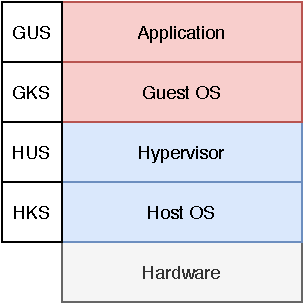
\includegraphics[width=\textwidth]{components-vm}
        \caption{Τυπικό \en{VM}}
        \label{fig:components-vm}
    \end{subfigure}
    \begin{subfigure}[b]{0.3\textwidth}
        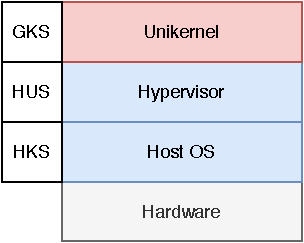
\includegraphics[width=\textwidth]{components-unikernel}
        \caption{\en{Unikernel}}
        \label{fig:components-unikernel}
    \end{subfigure}
    \begin{subfigure}[b]{0.3\textwidth}
        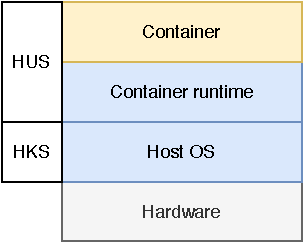
\includegraphics[width=\textwidth]{components-container}
        \caption{\en{Container}}
        \label{fig:components-container}
    \end{subfigure}
    \caption[Σύγκριση μεταξύ αρχιτεκτονικής ``κλασικής'' εικονικής μηχανής,
        \en{unikernel} και \en{container}]{Σύγκριση μεταξύ αρχιτεκτονικής
        ``κλασικής'' εικονικής μηχανής, \en{unikernel} και \en{container}, με
        \en{hypervisor} τύπου 2. Όπου \en{HKS=Host Kernel Space, HUS=Host User
        Space, GKS=Guest Kernel Space} και \en{GUS=Guest User Space}.}
    \label{fig:vm-unikernel-container}
\end{figure}

Μία σύγχρονη προσπάθεια αντιμετώπισης του προηγούμενου προβλήματος είναι τα
\en{unikernels} \cite{mirageos}. Αυτά είναι εκτελέσιμες εικόνες μηχανών
(\en{machine images}) που αποτελούνται από μία εφαρμογή μαζί με όλες τις
απαραίτητες εξαρτήσεις (\en{dependencies}) για την εκτέλεση της, από βιβλιοθήκες
και \en{runtime systems} έως υλοποιήσεις στοίβας δικτύωσης και οδηγούς συσκευών.
Όλα τα παραπάνω βρίσκονται σε έναν κοινό, επίπεδο χώρο διευθύνσεων, χωρίς
διάκριση σε \en{kernel} και \en{user space}, όπως φαίνεται και στο σχήμα
\ref{fig:components-unikernel}. Πρόκειται συνεπώς για ειδικού σκοπού πυρήνες,
κατασκευασμένους ώστε να τρέχουν μία μόνο εφαρμογή, εντός μίας εικονικής
μηχανής, κατόπιν της παρατήρησης ότι συχνά τα \en{virtual machines}
χρησιμοποιούνται για να εξυπηρετήσουν αποκλειστικά μία εφαρμογή.

Τα \en{unikernels} χτίζουν πάνω στην παλαιότερη ιδέα των \en{library operating
systems (OS)}, τα οποία περιγράφονται μαζί με τα πολύ προοδευτικά για την εποχή
τους και επίκαιρα σήμερα \en{exokernels} \cite{exokernel}.
Σε ένα \en{library OS}, η πλειονότητα των λειτουργιών που παραδοσιακά
προσφέρονται ως μέρος ενός μονολιθικού πυρήνα, όπως το σύστημα αρχείων και η
στοίβα δικτύωσης, εξάγονται από αυτόν και γίνονται ανεξάρτητα στοιχεία με την
μορφή βιβλιοθηκών, οι οποίες συνοδεύουν την εφαρμογή. Αυτή η αναδιαμόρφωση
επιτρέπει στην εφαρμογή ελευθερία επιλογής ως προς το ποια από αυτά τα στοιχεία
χρειάζεται να συμπεριλαμβάνει αλλά και ως προς τη συγκεκριμένη υλοποίηση που θα
χρησιμοποιήσει για κάθε ένα από αυτά. Συνεπώς, η εφαρμογή δύναται να
βελτιστοποιήσει τη λειτουργία της μέσω των παραπάνω επιλογών, αλλά ταυτόχρονα
επιβαρύνεται από αυτή την επιπλέον ευθύνη.

Ένα μεγάλο εμπόδιο στην υλοποίηση των \en{unikernels} είναι η ποικιλία συσκευών
και κατά συνέπεια οδηγών που χρειάζονται για την υποστήριξη τους. Αυτό
ξεπερνιέται χάρη στο μοντέλο συσκευών των \en{hypervisors}, το οποίο
περιλαμβάνει λίγες, κοινές και καλώς καθορισμένες συσκευές. Ένα άλλο εμπόδιο
είναι η πολυπλοκότητα της διαδικασίας ταιριάσματος των διαφορετικών στοιχείων
(\en{components}) μεταξύ τους και της κατασκευής της τελικής εκτελέσιμης εικόνας
από αυτά. Για την αντιμετώπιση του διατίθεται πληθώρα λύσεων, με κάθε μία
να σχηματίζει ένα λεγόμενο \en{unikernel framework}. Πρακτικά όλα αυτά είναι
έργα ελεύθερου λογισμικού, με καθένα να προσφέρει συνήθως ένα σύνολο
βιβλιοθηκών για χρήση από τις εφαρμογές των χρηστών, όπως επίσης και τα
απαραίτητα εργαλεία για το χτίσιμο των εικόνων. Κάθε ένα από αυτά τα
\en{frameworks} ακολουθεί τυπικά μία από δύο βασικές προσεγγίσεις:
\begin{itemize}
    \item Αγνή (\en{clean-slate}), που χαρακτηρίζεται από την παροχή
        μη-πρότυπων (\en{custom}) διεπαφών εφαρμογής (\en{APIs}). Επίσης, σε
        αυτή την περίπτωση ο κώδικας των βιβλιοθηκών αλλά και της εφαρμογής
        είναι γραμμένος στην ίδια γλώσσα. Σαφές μειονέκτημα αποτελεί το γεγονός
        ότι οι εφαρμογές πρέπει να γραφτούν από την αρχή στη γλώσσα και με χρήση
        του \en{API} του εκάστοτε \en{framework}.
    \item Συμβατή (\en{compatible}), που χαρακτηρίζεται από την παροχή
        παραδοσιακών διεπαφών (πχ \en{POSIX}), επιτρέποντας σε ήδη υπάρχουσες
        εφαρμογές να εκτελεστούν με ελάχιστες έως καθόλου τροποποιήσεις,
        ανεξάρτητα από τη γλώσσα στην οποία έχουν αρχικά γραφτεί (\en{binary
        compatibility}). Εν προκειμένω, το μεγαλύτερο μειονέκτημα είναι η
        δέσμευση με συχνά παλαιωμένες διεπαφές, που δεν επιτρέπουν την πλήρη
        εκμετάλλευση του δυναμικού των \en{unikernels}.
\end{itemize}
Ενδεικτικά, στην πρώτη κατηγορία ανήκουν το \en{MirageOS} \cite{mirageos} και το
\en{IncludeOS} \cite{includeos}, ενώ στη δεύτερη βρίσκει κανείς τα \en{RumpRun}
\cite{rumprun}, \osv{} \cite{osv} και \en{HermiTux} \cite{hermitux}. Συνολικά
υπάρχει ένας αρκετά μεγάλος αριθμός \en{unikernel frameworks}. Η δημοτικότητα
τους κυμαίνεται, χωρίς κάποιο να επικρατεί, ενώ ποικίλουν τα στάδια συντήρησης
τους (από ενεργά έως πρακτικά εγκαταλελειμμένα) όπως και οι καταβολές τους
(ακαδημαϊκά, εταιρικά ή και προσωπικά έργα).

% TODO OPT: Mention edge use case for unikernels? (not here necessarily)

\subsection{\osv{}}
Το \osv{} είναι ένα \en{unikernel framework} που υποστηρίζει εφαρμογές γραμμένες
για το \linux{}, ενώ παρέχει και δικό του \en{API}, το οποίο μπορούν
προαιρετικά να χρησιμοποιήσουν νέες εφαρμογές \cite{osv}. Εξ' αρχής σχεδιάστηκε
με το \en{cloud} κατά νου, προκειμένου να χρησιμοποιηθεί ιδίως από σύγχρονες
εφαρμογές που συχνά συναντώνται σε αυτό. Ως έργο ξεκίνησε από την \en{Cloudius
Systems} (μετέπειτα \en{ScyllaDB}), αλλά τα τελευταία χρόνια συντηρείται εξ'
ολοκλήρου από μία μικρή ομάδα εθελοντών, ενώ είναι διαθέσιμο με τους όρους της
άδειας \en{BSD}. Η κοινότητα του χρησιμοποιεί μία \en{mailing list}%
\footnote{\en{\url{https://groups.google.com/forum/\#!forum/osv-dev}}}
για την ανάπτυξη του: υποβολή \en{patches}, \en{code review} και γενική
συζήτηση.

Αν και τα κομμάτια που παρέχει το ίδιο είναι γραμμένα σε \en{C++}, ενώ
χρησιμοποιεί κομμάτια από άλλα έργα που ως επί το πλείστον έχουν γραφτεί σε
\en{C}, δεν θέτει περιορισμούς στις εφαρμογές που υποστηρίζει. Το
τελευταίο βέβαια ισχύει αρκεί αυτές να μην κάνουν χρήση λειτουργιών που από τη
φύση τους δεν υλοποιούνται στα \en{unikernels}: κλήσεις συστήματος στην
οικογένεια των \texttt{\en{fork()}} και \texttt{\en{exec()}}. Επίσης, διαθέτει
υποστήριξη για πολλούς \en{hypervisors}, μεταξύ των οποίων οι \qemu{}/\en{KVM},
\en{Xen} και \en{firecracker} \cite{firecracker}.
Ως γενική παρατήρηση, είναι από τα πλέον εξελιγμένα \en{unikernels} από πλευράς
λειτουργιών, και πιο ``βαρύ'' (\en{heavy-weight}) κατά συνέπεια.

Συγκεκριμένα όσον αφορά τα συστήματα αρχείων, το \osv{} προσφέρει πολλές
επιλογές. Κατ' αρχάς, διαθέτει ένα ολοκληρωμένο εικονικό σύστημα αρχείων
(\en{VFS, Virtual File System}), το οποίο έχει βασίσει σε αυτό του \en{Prex}
\cite{prex}.
Κάτω από αυτό βρίσκονται οι υλοποιήσεις των διάφορων συστημάτων αρχείων που
διαθέτει, τα οποία διακρινόμενα σε δύο κατηγορίες είναι:
\begin{itemize}
    \item Τα \en{pseudo-file systems}, αντίστοιχα με αυτά στο \linux{}:
        \en{devfs, procfs, sysfs} και \en{ramfs}.
    \item Τα συμβατικά συστήματα αρχείων: \en{ZFS} (βασισμένο σε υλοποίηση του
        \en{FreeBSD}), \en{rofs} (\en{custom, read-only file system} με απλή
        λογική \en{caching}) και \en{NFS} (χρησιμοποιώντας τη \en{libnfs}
        \cite{libnfs}).
\end{itemize}

% TODO OPT: More technical: virtual memory, virtual file system, network stack,
% aarch64, musl.

\subsection{Εναλλακτικές}
Όπως είναι αναμενόμενο, έχουν προταθεί και εναλλακτικές προσεγγίσεις στο
πρόβλημα του \en{bloated virtualized software stack}. Με διαφορά η πιο
διαδεδομένη αυτήν την περίοδο είναι εκείνη των \en{containers}. Αυτά ανήκουν
στην ευρεία κατηγορία της εικονικοποίησης σε επίπεδο λειτουργικού συστήματος
(\en{OS-level virtualization} \cite{wiki:os-level-virtualization}, σχηματικά στο
\ref{fig:components-container}).

Υπάρχουν πολλές τεχνικές υλοποίησης των \en{containers}, οι περισσότερες εκ των
οποίων βασίζονται σε μηχανισμούς του \linux{} \en{kernel} όπως τα \en{cgroups}
και \en{namespaces} προκειμένου να παρέχουν απομόνωση μεταξύ των διαφορετικών
\en{containers}. Το κοινό όλων τους είναι ότι οι εφαρμογές που τρέχουν σε όλα
τα \en{containers} του ίδιου μηχανήματος μοιράζονται το ίδιο στιγμιότυπο πυρήνα
(\en{kernel}). Θα μπορούσαμε να πούμε ότι σε αυτή την περίπτωση έχουμε ένα
\en{kernel}, αλλά πολλαπλά \en{user spaces}.

Στα σημαντικά πλεονεκτήματα των \en{containers} είναι ότι είναι πολύ πιο
``ελαφριά'' από τις εικονικές μηχανές: πολύ χαμηλότερος χρόνος εκκίνησης (από
ένα \en{virtual machine} με \guest{} γενικού σκοπού), σε συνδυασμό με μεγαλύτερη
ευελιξία και πιο αποδοτική χρήση των πόρων, με αποτέλεσμα να μπορούν να
επιτύχουν υψηλότερη πυκνότητα (στιγμιότυπα που εκτελούνται ταυτόχρονα στο ίδιο
φυσικό μηχάνημα). Το σημαντικότερο μειονέκτημα τους είναι ότι προσφέρουν κατ'
αρχήν πολύ πιο ασθενή απομόνωση από ότι οι εικονικές μηχανές, λόγω του κοινού
πυρήνα που τα εξυπηρετεί απευθείας \cite{lightvm}.

% TODO OPT: Αll other approaches (lw virt, user-space kernels).

% TODO OPT: Compare native, legacy virtual, unikernel and container execution in
% terms of flexibility, security (separation) and efficiency / scalability.

\section{Κοινόχρηστα συστήματα αρχείων}
Τα ``κλασικά'' συστήματα αρχείων είναι υλοποιημένα πάνω από συσκευές \en{block}
(``δίσκους''), συνδεδεμένες μέσω ενός διαύλου (\en{bus}) τοπικού συστήματος.
Το λογισμικό που τα υλοποιεί είναι συνήθως μέρος του πυρήνα ενός λειτουργικού
συστήματος, το οποίο θεωρεί ότι έχει την αποκλειστικότητα επί του συστήματος
αρχείων από τη στιγμή της προσάρτησης (\en{mount}) μέχρι και την στιγμή της
αποπροσάρτησης (\en{unmount}) αυτού. Το τελευταίο αποτελεί σε πολλές περιπτώσεις
έναν περιορισμό, ο οποίος ήδη από την έλευση της δικτύωσης των υπολογιστών
επιδιώχθηκε να αρθεί, επιτρέποντας την ταυτόχρονη χρήση ενός συστήματος αρχείων
από περισσότερους υπολογιστές, καθιστώντας το κοινό. Ο πιο γνωστός και μεταξύ
των παλαιότερων εκπροσώπων κοινόχρηστων συστημάτων αρχείων είναι το \en{NFS
(Network File System)} \cite{nfs},
ενώ η κατηγορία έχει εμπλουτιστεί σημαντικά με την επέκταση των κατανεμημένων
υπολογιστικών συστημάτων τις τελευταίες δεκαετίες.

Με την εικονικοποίηση έχουμε μία ιδιαίτερη περίπτωση πολλαπλών, συνδεδεμένων
μηχανημάτων: του \host{} και των \en{virtual machines} που εκτελούνται σε αυτόν.
Το ζητούμενο του κοινόχρηστου συστήματος αρχείων μεταξύ τους είναι συνεπώς κι
εδώ παρόν και μάλιστα, λόγω της συνύπαρξης στο ίδιο φυσικό μηχάνημα είναι μία
πολύ συχνή απαίτηση. Εξάλλου, το σύστημα αρχείων στον \host{} αποτελεί έναν
ακόμα πόρο του, οπότε είναι αναμενόμενο να μπορεί να δοθεί πρόσβαση σε αυτόν από
τους \en{guests}.

Οι περισσότερες λύσεις για κοινόχρηστα συστήματα αρχείων μεταξύ \host{} και
\guest{} βασίζονται στα ήδη υπάρχοντα, δικτυακά συστήματα αρχείων, μη
διακρίνοντας αυτή την περίπτωση από εκείνη των χωριστών \en{hosts}. Αυτή η
προσέγγιση λειτουργεί βεβαίως βασιζόμενη στη σύνδεση δικτύου μεταξύ των μερών,
πλήρως επαναχρησιμοποιώντας ήδη υπάρχουσες λύσεις. Ένα δημοφιλές παράδειγμα
κοινόχρηστου συστήματος αρχείων στο πλαίσιο της εικονικοποίησης είναι το
\en{VirtFS} \cite{virtfs}, που εκμεταλλεύεται το πρωτόκολλο \en{9P} \cite{9p}.
Αν και το τελευταίο είναι ένα δικτυακό πρωτόκολλο, στην πράξη το \en{VirtFS}
δεν χρησιμοποιεί το δίκτυο στο επίπεδο μεταφοράς του, κάτι που του επιτρέπει
βελτιωμένες επιδόσεις.

Αξίζει να αναφέρουμε ότι και στην περίπτωση των \en{containers} είναι ιδιαίτερα
συχνή η απαίτηση της πρόσβασης σε κοινό σύστημα αρχείων με τον \host{}. Ένας
τρόπος με τον οποίο αυτό επιτυγχάνεται στο \en{Docker} \cite{docker}
(με διαφορά το πιο δημοφιλές \en{container runtime}) είναι η χρήση των λεγόμενων
\en{bind mounts} \cite{docker:bind-mounts},
που εκμεταλλεύονται τον κοινό πυρήνα για να προσαρτήσουν έναν κατάλογο του
\host{} εντός του συστήματος αρχείων του \en{container}.

\section{\viofs{}}
Η κοινή υποκείμενη μνήμη ανάμεσα στον \host{} και τους \en{guests} είναι ένα
στοιχείο το οποίο δεν εκμεταλλεύονται πλήρως τα υπάρχοντα κοινόχρηστα συστήματα
αρχείων. Αυτό έρχεται να αλλάξει το \viofs{} \cite{virtiofs-website}, το οποίο
έχει σχεδιαστεί εξ' αρχής με ετούτο το σκοπό. Το στοιχείο που το διαφοροποιεί
από τα υπόλοιπα είναι ότι δεν εξαρτάται από το δίκτυο στο επίπεδο μεταφοράς,
όπου χρησιμοποιεί το \en{virtio}, ούτε όμως και στο επίπεδο του πρωτοκόλλου,
όπου βασίζεται στο \en{FUSE}. Αυτές οι δύο επιλογές του επιτρέπουν καλύτερες
επιδόσεις, αλλά και σημασιολογία (\en{semantics}) τοπικού συστήματος αρχείων,
μια διαφορά που εκδηλώνεται για παράδειγμα σε θέματα συνοχής (\en{coherence}).

Η υπάρχουσα υλοποίηση του \viofs{} στο \qemu{} έχει μία αρχιτεκτονική
ιδιαιτερότητα. Ενώ τυπικά η υλοποίηση των συσκευών περιέχεται εξ' ολοκλήρου στο
\qemu{}, εδώ ένα σημαντικό μέρος της υλοποίησης είναι διαχωρισμένο, υλοποιημένο
στο λεγόμενο \en{virtiofsd (virtio-fs daemon)}, μία ανεξάρτητη διεργασία που
αναλαμβάνει όλες τις λειτουργίες του συστήματος αρχείων στον \host{}, ενώ το
\qemu{} έχει μόνο την ευθύνη της εικονικής συσκευής. Αυτή η αρχιτεκτονική
έχει αφενός το όφελος υψηλότερης ασφάλειας, καθώς ο \en{virtiofsd} μπορεί
περιοριστεί σε ένα \en{sandbox} χρησιμοποιώντας μηχανισμούς του \host{}
(\en{namespaces, seccomp}). Αφετέρου, είναι αρθρωτή (\en{modular}), επιτρέποντας
εύκολη εναλλαγή ανάμεσα σε διαφορετικές υλοποιήσεις του \en{virtiofsd} (πχ με
μία που αντί πρόσβασης στο σύστημα αρχείων του \host{} να χρησιμοποιεί κάποιο
κατανεμημένο σύστημα αρχείων). Ο διαχωρισμός της υλοποίησης σε περισσότερες
διεργασίες καθίσταται δυνατός χάρη στο \en{vhost-user} πρωτόκολλο
\cite{vhost-user},
το οποίο με τη σειρά του εξελίσσει την ιδέα του \en{vhost} στο \qemu{}
\cite{stefanha:vhost}. Η ώθηση των συσκευών εκτός του \en{VMM} έχει αρκετά
πλεονεκτήματα και είναι μία τάση που αναμένεται να ακολουθηθεί και στο μέλλον
\cite{stefanha:out-of-process-dev}.

\subsection{\en{Virtio}}
Το \en{virtio} είναι μία πρότυπη (\en{standard}) προδιαγραφή συσκευών,
αποκλειστικά για \en{virtualized} περιβάλλοντα \cite{virtio}. Χαίρει ευρείας
υποστήριξης και είναι η πλέον αποδεκτή λύση στο πρόβλημα του κατακερματισμού
(\en{fragmentation}) των μοντέλων συσκευών σε αυτά. Προσφέρει έναν αποδοτικό και
επεκτάσιμο μηχανισμό, ενώ βασίζεται σε ορολογία και μηχανισμούς φυσικών
συσκευών, διευκολύνοντας την υποστήριξη και επιτρέποντας την επαναχρησιμοποίηση
από υπάρχουσες υλοποιήσεις οδηγών στους \en{guests}.

Το πρότυπο έχει δύο βασικούς άξονες:
\begin{description}
    \item[Το επίπεδο μεταφοράς] το οποίο ορίζει έναν γενικό τρόπο για την
        ανακάλυψη (\en{discovery}), διαμόρφωση (\en{configuration}) και κανονική
        λειτουργία (αμφίδρομη μεταφορά δεδομένων) των συσκευών. Η τελευταία
        γίνεται μέσω των λεγόμενων \en{virtqueues}, βασιζόμενη στην κοινή μνήμη
        μεταξύ \guest{} και \en{hypervisor}. Το επίπεδο μεταφοράς, το οποίο
        κατ' αρχήν ορίζεται αφηρημένα, εξειδικεύεται με τρεις υλοποιήσεις:
        δίαυλο \en{(bus) PCI}, \en{memory-mapped I/O (MMIO)} και \en{channel
        I/O} (για περιπτώσεις βασισμένες στην αρχιτεκτονική \en{S/390} της
        \en{IBM}).
    \item[Το σύνολο των συσκευών] που χτίζεται πάνω από το επίπεδο μεταφοράς,
        καθορίζοντας για κάθε συσκευή τα διαθέσιμα πεδία διαμόρφωσης
        (\en{configuration fields}) της, το πλήθος των \en{virtqueues} που
        χρησιμοποιεί και τα μηνύματα που μεταφέρονται μέσω αυτών για τη
        λειτουργία της.
\end{description}

\subsection{\en{FUSE}}
Το \en{FUSE (Filesystem in Userspace)} είναι ένα πρωτόκολλο που συστήθηκε στο
\linux{} προκειμένου να επιτρέψει την υλοποίηση συστημάτων αρχείων στο
\en{user space} αντί εντός του πυρήνα \cite{fuse}.
Όπως φαίνεται και στο σχήμα \ref{fig:fuse}, στην αρχιτεκτονική του η υλοποίηση
των λειτουργιών του συστήματος αρχείων γίνεται από ένα \en{user space daemon}
που επικοινωνεί σύμφωνα με το πρωτόκολλο με τον πυρήνα μέσω μίας ειδικής
συσκευής χαρακτήρων (\texttt{\en{/dev/fuse}}). Όταν το \en{kernel} δέχεται
\en{VFS} αιτήματα που αντιστοιχούν σε κάποιο \en{FUSE} σύστημα αρχείων, τα
προωθεί στο κατάλληλο \en{daemon}, που έχει το ρόλο του \en{backend}.

\begin{figure}
    \centering
    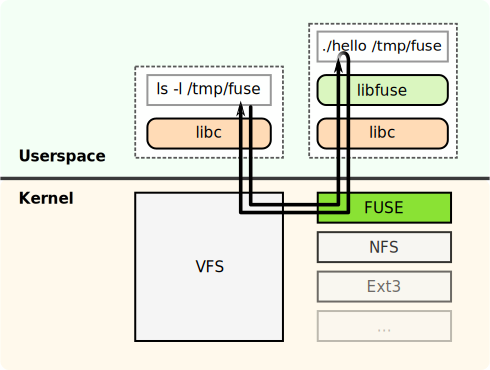
\includegraphics[width=\textwidth]{fuse}
    \caption[Δομή του \en{FUSE} στο \linux{}]{Δομή του \en{FUSE} στο
        \linux{}. Από τον \en{Sven}
        (\en{\url{https://commons.wikimedia.org/wiki/User:Sven}}) υπό την άδεια
        \en{CC-BY-SA 3.0}
        (\en{\url{https://creativecommons.org/licenses/by-sa/3.0/legalcode}}).
        Πηγή
        \en{\url{https://commons.wikimedia.org/wiki/File:FUSE_structure.svg}}.}
    \label{fig:fuse}
\end{figure}

Στο πλαίσιο του \viofs{}, το \en{FUSE} αξιοποιείται ως πρωτόκολλο επικοινωνίας
των αιτημάτων συστήματος αρχείων με τη συσκευή. Έτσι, κατά κάποιον τρόπο η
αρχιτεκτονική του μοιάζει με την κλασική αρχιτεκτονική του \en{FUSE} με τη
διαφορά ότι πελάτης (\en{client}) είναι ο \en{guest} αντί του πυρήνα, ενώ η
επικοινωνία γίνεται μέσω \en{virtio} αντί της \en{FUSE} συσκευής χαρακτήρων.
Στην πράξη όμως, το \viofs{} και το τυπικό \en{FUSE} είναι ασύμβατα μεταξύ τους,
με το \viofs{} να περιλαμβάνει τροποποιήσεις και επεκτάσεις στο πρωτόκολλο του
\en{FUSE}. Επίσης, το μοντέλο ασφαλείας (\en{security model}) είναι διαφορετικό
(ουσιαστικά ανεστραμμένο), μιας και στο \viofs{} ο \en{client} (\guest{}) είναι
αναξιόπιστος, ενώ στο \en{FUSE} συμβαίνει το αντίθετο (υπάρχει εξ' ορισμού
εμπιστοσύνη στον πυρήνα πάνω στον οποίο τρέχει ο \en{daemon}). Το τελευταίο
μεταφράζεται σε πιο ασφαλή χειρισμό των αιτημάτων σε ένα \viofs{} \en{device
backend} από ότι σε ένα \en{FUSE backend}.

% TODO OPT: Protocol description

\subsection{\en{DAX window}}
Ο τρόπος που διαθέτει το \en{FUSE} για την ανάγνωση και εγγραφή αρχείων είναι
μέσω των \en{FUSE\_READ} και \en{FUSE\_WRITE requests} αντίστοιχα. Αυτά
προβλέπουν την αντιγραφή των δεδομένων και, στην περίπτωση του \viofs{}
συνεπάγονται και εξόδους της εικονικής μηχανής (\en{VM exits}). Καθώς όμως αυτές
οι δύο λειτουργίες είναι κεντρικές στο \en{data path}, η βελτιστοποίηση τους
είναι απαραίτητη. Προς αυτή την κατεύθυνση το \viofs{} συστήνει το λεγόμενο
\en{DAX window}: ένα ``παράθυρο'' κοινής μνήμης ανάμεσα στον \host{} και το
\guest{}, στο οποίο απεικονίζονται τα περιεχόμενα των αρχείων, δίνοντας στον
\guest{} απευθείας πρόσβαση σε αυτά. Με αυτόν τον τρόπο επιτυγχάνεται αποφυγή
των αντιγραφών (και παράκαμψη της \en{page cache} του \en{guest} στην περίπτωση
του \linux{}), ενώ πλέον δεν συνεπάγεται κάθε λειτουργία ανάγνωσης ή εγγραφής
έξοδο από την εκτέλεση της εικονικής μηχανής.

\begin{figure}
    \centering
    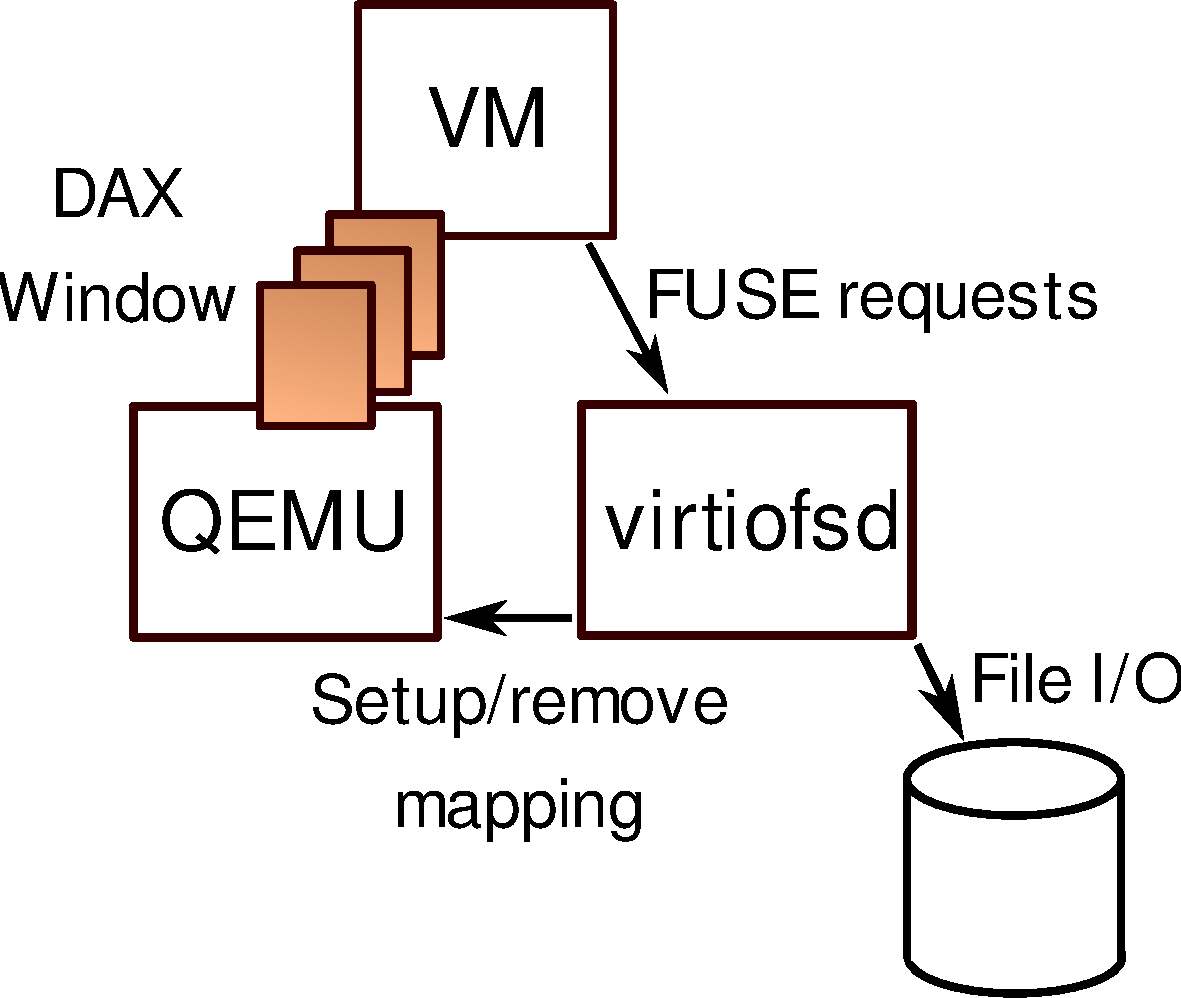
\includegraphics[scale=0.5]{dax-architecture}
    \caption[Αρχιτεκτονική του \en{DAX window} στο \viofs{}]{Αρχιτεκτονική του
        \en{DAX window} στο \viofs{}. Από τον \en{Stefan Hajnoczi}
        (\en{\url{https://vmsplice.net/}}) υπό την άδεια \en{CC-BY-SA 4.0}
        (\en{\url{https://creativecommons.org/licenses/by-sa/4.0/legalcode}}).
        Πηγή
        \en{\url{https://gitlab.com/virtio-fs/virtio-fs.gitlab.io/-/blob/master/architecture.svg}}.}
    \label{fig:dax-architecture}
\end{figure}

% TODO OPT: DAX subsystem in Linux, pmem

Για την υλοποίηση της λειτουργικότητας του \en{DAX window} κατ' αρχάς
επεκτείνεται το \en{FUSE} πρωτόκολλο με μηνύματα για την εγκαθίδρυση και την
κατάργηση απεικονίσεων (\en{mappings}). Αυτά τα μηνύματα χρησιμοποιεί ο \guest{}
προκειμένου ο \en{virtiofsd} (κατόπιν των απαραίτητων ελέγχων) να καθοδηγήσει το
\qemu{} μέσω της μεταξύ τους σύνδεσης να πραγματοποιήσει καθεαυτή τη λειτουργία
(δημιουργία ή κατάργηση απεικόνισης). Σχηματικά τα παραπάνω φαίνονται
στο \ref{fig:dax-architecture}.

\chapter{Υλοποίηση}

% TODO OPT: Note that we had set off to implement it from scratch but were
% working in parallel due to miscommunication?
Μία βασική υλοποίηση-σκελετός του \viofs{} υπήρχε στο \osv{}. % ref https://github.com/cloudius-systems/osv/commit/bae4381d1d0558b7a684294e9203864f9652395c
Αυτή υποστήριζε
απλή (μέσω της κλήσης \en{FUSE\_READ}) ανάγνωση αρχείων (και όχι καταλόγων).
Σε συνεννόηση με τα υπόλοιπα μέλη της κοινότητας του \osv{}, θέσαμε στόχο να
αναπτύξουμε περαιτέρω τη λειτουργικότητα αυτής της υλοποίησης. Το κομβικό
σημείο αυτής της προσπάθειας ήταν η υποστήριξη ανάγνωσης μέσω του \viofs{}
\en{DAX window}, κάτι που είχε σχεδιαστεί και υλοποιηθεί (σε "πειραματικό" ακόμα
στάδιο) από τους ανθρώπους του \viofs{} με σκοπό την δραματική βελτίωση των
επιδόσεων του συστήματος αρχείων. Εκτός αυτού, είχαμε την ευκαιρία να
προσθέσουμε υποστήριξη για ανάγνωση καταλόγων, καθώς και εκκίνηση (\en{boot})
του \osv{} με το \viofs{} ως ριζικό (\en{root}) σύστημα αρχείων. Στην πορεία
απαιτήθηκαν δομικές αλλαγές, διορθώσεις και βελτιώσεις στην προϋπάρχουσα
υλοποίηση.

Σε αυτό το κεφάλαιο αναλύουμε την υλοποίηση των πιο ουσιαστικών από τις παραπάνω
συμβολές: της ανάγνωσης αρχείων μέσω \en{DAX window} και του \en{boot} από
\viofs{}.

\section{\en{DAX window} στο \viofs{}}

Το \osv{} ακολουθεί μία εσωτερική δομή συμβατή με αυτή των περισσότερων πυρήνων
γενικού σκοπού, ορίζοντας χωριστά τις έννοιες του οδηγού (\en{driver}) και του
συστήματος αρχείων. Οι οδηγοί (στο \en{drivers/}) είναι υπεύθυνοι για
την παροχή μίας διεπαφής (\en{interface}) κοινής για κάθε οικογένεια συσκευών
(αποθήκευσης \en{block}, δικτύου κλπ), η οποία επιτρέπει τη χρήση της εκάστοτε
συσκευής από τα υπόλοιπα υποσυστήματα του πυρήνα. Τα συστήματα αρχείων (στο
\en{fs/}) αποτελούν επίσης υλοποιήσεις μίας κοινής διεπαφής η οποία ορίζεται από
το εικονικό σύστημα αρχείων (\en{virtual file system}) του \osv{}. Αυτή η
διεπαφή αποτελείται από λειτουργίες όπως το άνοιγμα, το κλείσιμο, η ανάγνωση από
αρχείο, και άλλες. Τα συστήματα αρχείων συνήθως είναι υλοποιημένα πάνω από μία
συσκευή \en{block} και χρησιμοποιούν τη διεπαφή που αυτή παρέχει για να
``μεταφράσουν'' ανάμεσα στις υψηλού επιπέδου λειτουργίες του συστήματος αρχείων
και τις χαμηλού επιπέδου λειτουργίες της συσκευής αποθήκευσης. Υπάρχουν βεβαίως
εξαιρέσεις όπως το \en{NFS}, το οποίο υποστηρίζεται από το δικτυακό υποσύστημα.

Το \viofs{} είναι ιδιαίτερο στο γεγονός ότι, ως σύστημα αρχείων εξαρτάται από
την ομώνυμη συσκευή, η οποία δεν μπορεί να αντιμετωπιστεί ως μέλος κάποιας από
τις συνήθεις οικογένειες (πχ \en{block} ή δικτύου). Αυτό το χαρακτηριστικό το
κληρονομεί βεβαίως από το \en{FUSE}. Έτσι, αναπόφευκτα υπάρχει ισχυρή, ρητή
εξάρτηση του \viofs{} συστήματος αρχείων από τον οδηγό της \viofs{} συσκευής,
κάτι που βλέπουμε και στην περίπτωση του \linux{}, όπου αυτά τα δύο είναι
υλοποιημένα μαζί (στο \en{fs/fuse/virtio\_fs.c}). Αυτό σημειώνεται ενόψει της
παρουσίασης της υλοποίησης που ακολουθεί, η οποία γίνεται υπό το πρίσμα της
διάκρισης ανάμεσα σε οδηγό και σύστημα αρχείων, αν και αυτή η διάκριση (δηλαδή
ο αντίστοιχος καταμερισμός των λειτουργιών) είναι εύκαμπτη.

\begin{figure}
    \centering
    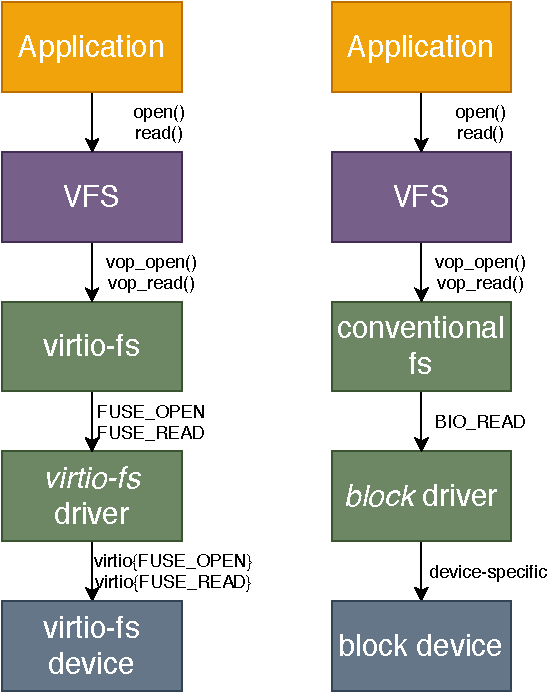
\includegraphics{virtiofs-vs-others}
    \caption{Συστατικά και εξαρτήσεις στον \guest{}: \viofs{} σε σύγκριση με
        συμβατικά συστήματα τοπικά αρχείων.}
    \label{fig:virtiofs-vs-others}
\end{figure}

\subsection{Οδηγός}

Ο οδηγός της \viofs{} συσκευής είναι επιφορτισμένος με την απευθείας επικοινωνία
και διαχείριση της. Πέρα από την αρχικοποίηση (ανακάλυψη \en{virtqueues},
διαπραγμάτευση παραμέτρων λειτουργίας) \cite{virtio}, το κύριο έργο του είναι η
μεταφορά αιτημάτων (\en{requests}) και απαντήσεων (\en{responses}) σε αυτά από
και προς τη συσκευή μέσω των \en{virtqueues}. Γι' αυτό το σκοπό παρέχει μία
ασύγχρονη διεπαφή υποβολής αιτημάτων, στα οποία ενθυλακώνονται τα \en{FUSE}
αιτήματα. Ο οδηγός παραμένει αγνωστικός ως προς το \en{FUSE}, χειριζόμενος τα
αιτήματα του ως αδιαφανή.

Η αρχικά διαθέσιμη υλοποίηση του \viofs{} \en{DAX window} στο \qemu{} ήταν ως
συσκευή \en{PCI}. Σύμφωνα με την προδιαγραφή του \en{virtio} \cite{virtio}
για τη συσκευή, το \en{DAX window} είναι η περιοχή κοινής μνήμης (\en{shared
memory region}) με αναγνωριστικό (``\en{shmid}'') 0. Στην περίπτωση του
\en{virtio PCI transport}, οι περιοχές κοινής μνήμης υλοποιούνται ως
\en{PCI BARs (base address registers)}, κάθε ένα εκ των οποίων εκτίθεται ως ένα
\en{VIRTIO\_PCI\_CAP\_SHARED\_MEMORY\_CFG PCI capability}, έχοντας ένα μοναδικό
αναγνωριστικό \cite{virtio} \cite{wiki:pci-conf} \cite{osdev:pci}.

Το πρώτο βήμα για την προσθήκη του \en{DAX window} ήταν λοιπόν η ανακάλυψη
(\en{discovery}) αυτού, εφόσον παρέχονταν από τη συσκευή. Αυτή ήταν μία ανώδυνη
εργασία, χάρη στο πλήρες και καλά μοντελοποιημένο υποσύστημα \en{PCI} του
\osv{}. Συγκεκριμένα, οι επιμέρους αλλαγές που χρειάστηκαν ήταν:
\begin{enumerate}
    \item Προσθήκη στο \en{PCI} υποσύστημα ώστε να είναι δυνατή η ανακάλυψη
          πολλαπλών \en{capabilities} με τον ίδιο τύπο (στο
          \en{drivers/pci-function.cc}). Αυτό ήταν απαραίτητο διότι μέχρι
          πρότινος οι λειτουργίες ανακάλυψης στο \osv{} αναζητούσαν μέχρι και το
          πρώτο \en{capability} ενός τύπου, σταματώντας εκεί. Όμως, όπως
          αναφέραμε προηγουμένως, κάθε περιοχή κοινής μνήμης αντιστοιχεί σε ένα
          \en{PCI capability} και αυτές μπορεί να είναι περισσότερες από μία (αν
          και στην περίπτωση του \viofs{} υπάρχει μόνο μία).
    \item Επέκταση στο μοντέλο των \en{virtio PCI} συσκευών (στο    % TODO OPT: Rephrase to avoid overfull hbox
          \en{drivers/virtio-pci-device.cc}) ώστε να ανακαλύπτει όλες τις
          περιοχές κοινής μνήμης κάθε συσκευής, αναζητώντας τα \en{capabilities}
          αντίστοιχου τύπου και αποθηκεύοντας τα στοιχεία (διεύθυνση και
          μέγεθος) των \en{BARs} που αυτά υποδεικνύουν.
    \item Επέκταση στον οδηγό της \viofs{} συσκευής (στο
          \en{drivers/virtio-fs.cc}) ώστε να ανακαλύπτει την περιοχή κοινής
          μνήμης με αναγνωριστικό 0, δηλαδή το \en{DAX window} και να το εκθέτει
          απευθείας στη διεπαφή του, ως περιοχή \en{MMIO (memory-mapped I/O)}
          της συσκευής. Σημειώνεται ότι η απεικόνιση (\en{mapping}) της περιοχής
          στον εικονικό χώρο διευθύνσεων έχει ήδη πραγματοποιηθεί από το μοντέλο
          της συσκευής.
\end{enumerate}

\subsection{Σύστημα αρχείων}

Το \viofs{} σύστημα αρχείων θεωρεί δεδομένο έναν μηχανισμό αποστολής \en{FUSE}
αιτημάτων (ο οποίος παρέχεται από τον οδηγό) και πάνω σε αυτόν χτίζει τη
λειτουργικότητα του. Αυτό είναι συνεπώς επιφορτισμένο με τη γνώση και τον
χειρισμό του περιεχομένου των αιτημάτων που ο οδηγός απλώς μεταφέρει.

\subsubsection{Απεικόνιση αρχείων}

Η προσάρτηση (\en{mounting}) ενός \viofs{} συστήματος αρχείων συνίσταται στην
έναρξη μίας \en{FUSE} συνεδρίας (\en{session}) με την αποστολή ενός
\en{FUSE\_INIT} αιτήματος (\en{request}) \cite{virtio}. Με αυτό πραγματοποιείται
η διαπραγμάτευση των παραμέτρων της συνεδρίας, μεταξύ των οποίων και μίας που
αφορά τη λειτουργία του \en{DAX window}: η ευθυγράμμιση των απεικονίσεων
(\en{map alignment}). Η πρώτη τροποποίηση που απαιτούνταν στο σύστημα αρχείων
λοιπόν ήταν η επέκταση της διαδικασίας προσάρτησης ώστε να γνωστοποιείται στη
συσκευή ότι υποστηρίζεται από το λειτουργικό το \en{DAX window} και να
λαμβάνεται η τιμή της παραμέτρου από την απάντηση.

Η παραπάνω παράμετρος περιορίζει τα \en{mappings} αρχείων στο \en{DAX window} ως
εξής: τόσο η μετατόπιση (\en{offset}) της αρχής ενός \en{mapping} μέσα στο
αρχείο όσο και στο \en{DAX window} πρέπει να είναι ευθυγραμμισμένες σύμφωνα με
το \en{map alignment}. Αυτό στην πράξη επιβάλλεται στην παρούσα υλοποίηση της
\viofs{} συσκευής από τη χρήση της \en{mmap} \cite{man:mmap} στον \host{}
(επίσης ο λόγος που το \en{map alignment} συνήθως ταυτίζεται με το μέγεθος της
σελίδας μνήμης στον \host{}).

Όπως ορίζεται από την προδιαγραφή, η παροχή του \en{DAX window} από τη συσκευή
όπως και η χρησιμοποίηση του από τον \guest{} είναι αμφότερα προαιρετικά.
Επίσης, η χρήση του \en{DAX window} είναι ανεξάρτητη από τη χρήση της συμβατικής
\en{FUSE\_READ} (που είναι πάντοτε διαθέσιμη) για την ανάγνωση αρχείων. Έτσι, η
υλοποίηση μας, εφόσον είναι διαθέσιμο το \en{DAX window}, επιχειρεί να
ικανοποιήσει όλες τις αναγνώσεις αρχείων μέσω αυτού. Σε περίπτωση όμως που αυτό
δεν είναι διαθέσιμο ή αποτύχει η διαδικασία της ανάγνωσης από εκείνο, στρέφεται
δυναμικά στην εφεδρική \en{FUSE\_READ}, όπως φαίνεται και στο διάγραμμα
\ref{fig:dax-flowchart}.

\begin{otherlanguage}{english}
\begin{lstlisting}[
    float,
    caption=\gr{Οι ορισμοί του \en{FUSE} για τις λειτουργίες απεικονίσεων.
        Βλέπε παράρτημα \ref{app:copyright} για σημείωμα πνευματικών
        δικαιωμάτων.},
    label=lst:fuse-defs,
    language=C,
    captionpos=b,
    frame=single,
    basicstyle=\ttfamily,
    commentstyle=\color{olive},
    keywordstyle=\color{blue}]
#define FUSE_SETUPMAPPING_FLAG_WRITE (1ull << 0)
struct fuse_setupmapping_in {
    /* An already open handle */
    uint64_t        fh;
    /* Offset into the file to start the mapping */
    uint64_t        foffset;
    /* Length of mapping required */
    uint64_t        len;
    /* Flags, FUSE_SETUPMAPPING_FLAG_* */
    uint64_t        flags;
    /* memory offset in to dax window */
    uint64_t        moffset;
};

struct fuse_removemapping_in {
    /* number of fuse_removemapping_one follows */
    uint32_t        count;
};

struct fuse_removemapping_one {
    /* Offset into the dax to start the unmapping */
    uint64_t        moffset;
    /* Length of mapping required */
    uint64_t        len;
};
\end{lstlisting}
\end{otherlanguage}

Για την εγκαθίδρυση ενός νέου \en{mapping}, το \viofs{} επεκτείνει το πρωτόκολλο
του \en{FUSE} συστήνοντας τη λειτουργία \en{FUSE\_SETUPMAPPING}. Ένα αίτημα
τέτοιου τύπου περιγράφεται από μία δομή (\en{struct})
\en{fuse\_setupmapping\_in} (ο ορισμός φαίνεται στον κώδικα
\ref{lst:fuse-defs}). Για την ακύρωση υπαρχόντων απεικονίσεων έχει προστεθεί η
\en{FUSE\_REMOVEMAPPING}, με το σώμα της να αποτελείται από ένα \en{struct
fuse\_removemapping\_in} ακολουθούμενο από το υποδεικνυόμενο πλήθος από
\en{struct fuse\_removemapping\_one}.

Τέλος, σημειώνουμε ότι σύμφωνα με την προδιαγραφή, ένα νέο \en{mapping} μπορεί
να ζητηθεί ενώ επικαλύπτει κάποιο υπάρχον. Εάν η κάλυψη είναι πλήρης, το
προϋπάρχον αντικαθίσταται από το νέο, ενώ αν επικαλύπτεται μερικώς, διασπάται.
Ένα αίτημα για νέο \en{mapping} μπορεί να αποτύχει σε περίπτωση εξάντλησης
πόρων της συσκευής, οπότε προτείνεται να δοκιμαστεί ξανά κατόπιν απελευθέρωσης
πόρων μέσω της ακύρωσης υπαρχουσών απεικονίσεων. Έτσι και στην υλοποίηση μας η
λειτουργία \en{FUSE\_REMOVEMAPPING} δεν χρησιμοποιείται υπό φυσιολογικές
συνθήκες.

\subsubsection{Διαχειριστής (\en{DAX window manager})}

Από τη δυνατότητα λεπτού ελέγχου των \en{DAX window mappings} που προσφέρεται,
προκύπτει το ζήτημα της βέλτιστης διαχείρισης του. Το τελευταίο έχει πολλά κοινά
με το πρόβλημα της διαχείρισης μνήμης στο πλαίσιο ενός λειτουργικού συστήματος
με σελιδοποίηση (\en{paging}), μιας και λόγω του \en{map alignment} οι
απεικονίσεις γίνονται πάντα σε όρους πολλαπλασίων αυτού. Για να το
αντιμετωπίσουμε λοιπόν χρειάστηκε να υλοποιήσουμε έναν διαχειριστή για το
\en{DAX window} στο επίπεδο του συστήματος αρχείων, μέσω του οποίου συμβαίνουν
όλες οι αναγνώσεις επιτρέποντας του να εφαρμόσει την πολιτική που περιγράφουμε
στη συνέχεια.

Για την διαμόρφωση της πολιτικής διαχείρισης λήφθηκαν υπόψη τα εξής:
\begin{itemize}
    \item Στην περίπτωση μας, το σύστημα αρχείων είναι μόνο για ανάγνωση
          (\en{read-only}).
    \item Το κόστος σε χρόνο ενός αιτήματος \en{FUSE\_SETUPMAPPING} είναι
          ανεξάρτητο του μεγέθους της απεικόνισης η οποία ζητείται.
    \item Μία σχετικά απλή πολιτική μεταφράζεται σε απλούστερη υλοποίηση,
          η οποία είναι ευκολότερο να είναι ορθή, αποδοτική και εύρωστη
          (\en{robust}).
\end{itemize}
Σύμφωνα με αυτά οδηγηθήκαμε σε ένα σχήμα διαχείρισης που συνοψίζεται από τα
παρακάτω χαρακτηριστικά (απεικονίζονται μερικώς και στο σχήμα
\ref{fig:dax-overview}):
\begin{itemize}
    \item Το \en{DAX window} χωρίζεται σε κομμάτια (\emph{\en{chunks}}) σταθερού
          μεγέθους (2 \en{MiB} από προεπιλογή). Αυτά αποτελούν τους δομικούς
          λίθους με την έννοια ότι όλες οι λειτουργίες (απεικονίσεις) γίνονται
          σε όρους αυτών των \en{chunks}. Κάθε νέο \en{mapping} λοιπόν ξεκινά
          από μία μετατόπιση εντός του αρχείου και εντός του \en{DAX window} που
          αμφότερες είναι πολλαπλάσια του μεγέθους του \en{chunk}, ενώ αφορά
          ακέραιο πλήθος \en{chunks}. Γίνεται έτσι σαφές ότι απαιτώντας το
          μέγεθος του \en{chunk} να είναι συμβατό με το \en{map alignment},
          αυτόματα ικανοποιούνται όλες οι απαιτήσεις ευθυγράμμισης που τίθενται
          από τη \viofs{} συσκευή. Αυτό επελέγη αφενός για απλότητα και αφετέρου
          ώστε να λειτουργεί (με την επιλογή του κατάλληλου μεγέθους \en{chunk})
          ως μονάδα προφόρτωσης (\en{prefetching}).
    \item Ένα νέο \en{mapping} ξεκινά πάντοτε από τη χαμηλότερη διαθέσιμη
          διεύθυνση εντός του \en{DAX window}. Εάν δεν υπάρχει αρκετός χώρος
          (το παράθυρο είναι γεμάτο), τότε γίνεται επικάλυψη με τις απεικονίσεις
          στις υψηλότερες διευθύνσεις, μόνο όσο χρειάζεται ώστε να χωρέσει η
          νέα. Έτσι, ακολουθείται το \en{LIFO (Last In - First Out)} μοντέλο,
          με το \en{DAX window} να προσιδιάζει μία στοίβα. Αυτό έγινε αφενός
          για απλότητα και αφετέρου ώστε στην περίπτωση μίας εφαρμογής που
          διαβάζει ένα αρχείο σειριακά με διαδοχικές κλήσεις, τα επιμέρους
          διαδοχικά \en{chunks} να βρίσκονται διατεταγμένα στο παράθυρο.
    \item Δεν γίνεται προφόρτωση (\en{prefetching}) των αρχείων πέρα του
          ενός \en{chunk}, προκειμένου να αποφευχθεί δυνητική σπατάλη του χώρου
          στο \en{DAX window}. Παρ' αυτά, σημειώνουμε ότι στην υλοποίηση
          περιλαμβάνεται η επιλογή (απενεργοποιημένη από προεπιλογή) για
          ``επιθετικό'' \en{prefetching}, όπου απεικονίζεται ολόκληρο το αρχείο
          με την πρώτη πρόσβαση σε αυτό.
\end{itemize}
Ολόκληρη η διαδικασία ανάγνωσης σε ότι αφορά την υλοποίηση του \viofs{}
απεικονίζεται ενδεικτικά με το διάγραμμα ροής \ref{fig:dax-flowchart}.

\begin{figure}
    \centering
    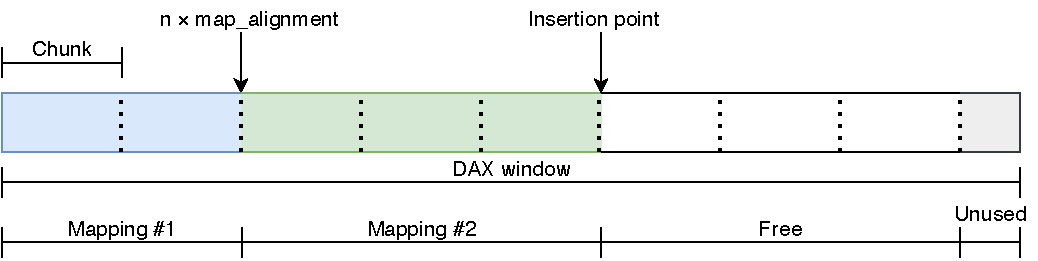
\includegraphics[width=\textwidth]{dax}
    \caption{Ενδεικτική εικόνα του \en{DAX window} υπό τον \en{manager}.}
    \label{fig:dax-overview}
\end{figure}

\begin{figure}
    \begin{minipage}[c][\textheight]{\textwidth}
        \centering
        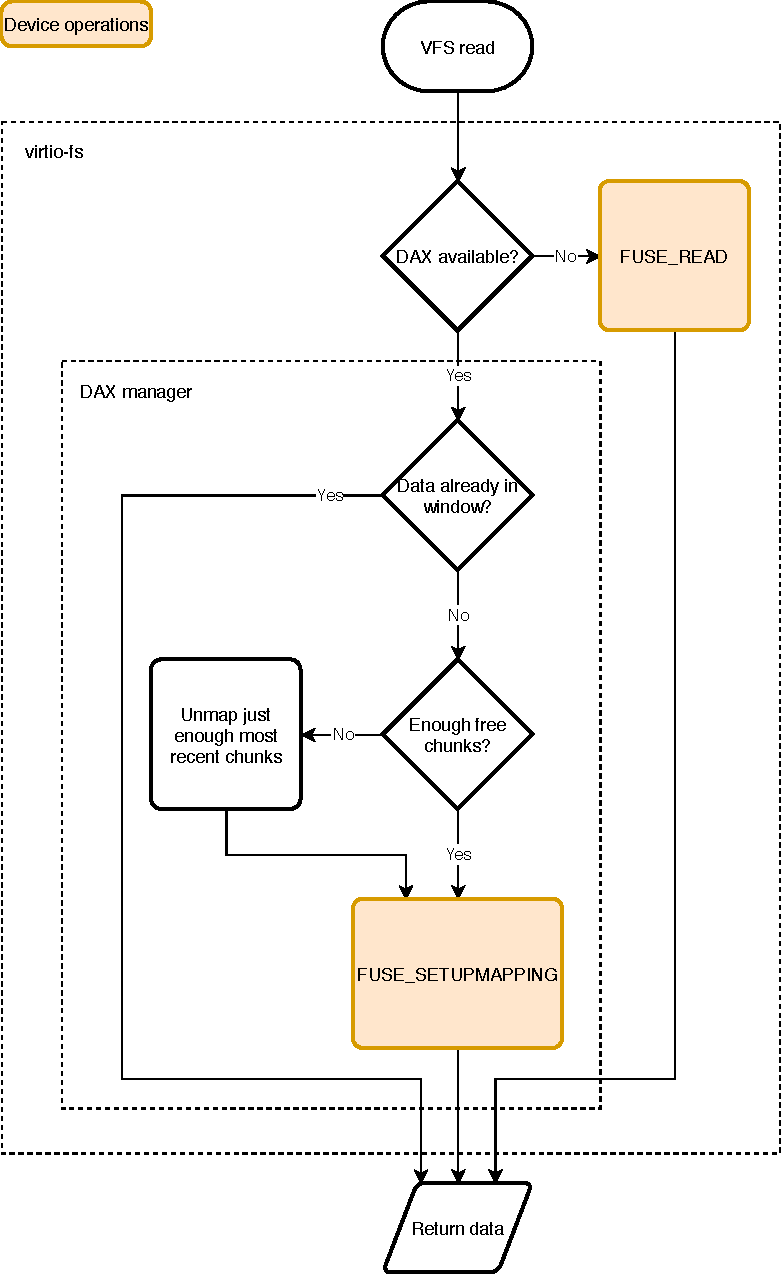
\includegraphics[height=\textheight]{read}
        \caption{Η διαδικασία ανάγνωσης από το \viofs{} υπό τον \en{manager}.}
        \label{fig:dax-flowchart}
    \end{minipage}
\end{figure}

\section{\en{Boot} από \viofs{}}

Η προσθήκη υποστήριξης για εκκίνηση (\en{boot}) από το \viofs{} στο \osv{}
είχε δύο συνιστώσες: την κυριότερη που αφορούσε τον πυρήνα του λειτουργικού
συστήματος αλλά και μία βοηθητική που αφορούσε τα εργαλεία αυτοματισμού για τη
δημιουργία και εκτέλεση των εικόνων. Αμφότερες βασίστηκαν σε προηγούμενες
αντίστοιχες επεκτάσεις, μιας και το \osv{} ήδη μπορούσε να χρησιμοποιήσει
είτε το \en{ZFS} είτε το \en{rofs} (και το \en{ramfs} βέβαια, που είναι
ιδιαίτερη περίπτωση) για το κύριο \en{root} σύστημα αρχείων του.

Συνοπτικά, τα σημεία που αφορούν το \en{root file system} κατά τον κύκλο ζωής
ενός \osv{} \en{unikernel}, όπως είχαν πριν την επέκταση μας είναι:
\begin{enumerate}
    \item Χτίσιμο της εικόνας (κεντρικό σημείο το \en{scripts/build}): σε αυτό
          το στάδιο επιλέγεται από τον χρήστη ο τύπος του συστήματος αρχείων
          και το \en{root file system} δημιουργείται με το περιεχόμενο που
          προκύπτει από την εφαρμογή. Επίσης, εδώ ξεκινά ο καθορισμός της
          εντολής εκκίνησης (\en{command line}) του \en{(uni)kernel}, η οποία
          περιέχει επιλογές για τον ίδιο τον πυρήνα, αλλά και το \en{command
          line} της εφαρμογής που πρόκειται να εκτελεστεί. Αυτή αποθηκεύεται
          σε ένα προσωρινό αρχείο, από όπου την παραλαμβάνει το επόμενο βήμα
          \cite{osv-wiki:osv-components}.
    \item Εκτέλεση της εικόνας (κεντρικό σημείο το \en{scripts/run.py}): εδώ
          προαιρετικά εμπλουτίζεται το \en{command line} με εφήμερες επιλογές
          πχ το επίπεδο λεπτομέρειας (\en{verbosity}) στα μηνύματα του πυρήνα.
          Κατόπιν, το ολοκληρωμένο \en{command line} εγγράφεται στο image,
          προτού αυτό εκτελεστεί.
    \item Φόρτωση του πυρήνα (κεντρικό σημείο το \en{loader.cc}): μετά από,
          μεταξύ άλλων, την αρχικοποίηση του πυρήνα, των συσκευών και των
          οδηγών, αλλά και το διάβασμα του \en{command line}, το \osv{}
          επιχειρεί να περάσει από το αρχικό, ενσωματωμένο σύστημα αρχείων του
          (\en{ramfs}) στο κύριο σύστημα αρχείων (\en{root file system})
          \cite{osv-wiki:osv-loader}. Αυτό συνίσταται στην προσάρτηση
          (\en{mounting}) του συστήματος αρχείων σε κάποιο σημείο του
          υπάρχοντος, αρχικού \en{ramfs}, ακολουθούμενη από το πέρασμα της ρίζας
          (\en{pivoting}) του εικονικού συστήματος αρχείων σε αυτό. Τα τελευταία
          γίνονται απλά, μέσω του εικονικού συστήματος αρχείων, αφού όλα τα
          προαπαιτούμενα για τη χρήση του έχουν ολοκληρωθεί.
\end{enumerate}
% TODO OPT: Diagram with build / run process and flow of relevant options.

Η επιλογή του συστήματος αρχείων που θα χρησιμοποιηθεί ως \en{root} κατά τη
φόρτωση μέχρι πρότινος ήταν δυναμική: γινόταν απόπειρα προσάρτησης από την
πρώτη συσκευή \en{block} αρχικά του \en{rofs} και εάν αυτό αποτύγχανε του
\en{ZFS}. Εάν αμφότερα αποτύγχαναν, η εκτέλεση συνεχιζόταν με το \en{ramfs}
αρχικό σύστημα αρχείων.
Αν και αυτή η διαδικασία θα μπορούσε εύκολα να επεκταθεί ώστε να συμπεριλάβει το
\viofs{}, γινόταν προφανές ότι βασιζόταν σε πολλές σιωπηλές υποθέσεις, χωρίς να
αφήνει μεγάλο περιθώριο ελέγχου στον χρήστη. Έτσι, αποφασίσαμε να κάνουμε ένα
πάμε ένα βήμα παραπέρα, ώστε να δοθεί περισσότερος έλεγχος επί της διαδικασίας:
προσθέσαμε μία επιλογή \texttt{\en{-{}-rootfs}} στη γραμμή εντολών του πυρήνα
(\en{command line option}), η οποία επιτρέπει να καθοριστεί ρητά ο τύπος του
\en{root file system} (ανάμεσα σε \en{ZFS, rofs}, \viofs{} και \en{ramfs}). Όπως
φαίνεται και στο διάγραμμα \ref{fig:rootfs}, αυτή η επιλογή είναι προαιρετική
και εάν δεν έχει καθοριστεί χρησιμοποιείται η παλαιότερη, δυναμική διαδικασία,
για συμβατότητα. Τέλος, κάναμε τις απαραίτητες αλλαγές στη διαδικασία χτισίματος
(\en{scripts/build}) ώστε να θέτει αυτή την επιλογή ανάλογα με το σύστημα
αρχείων που έχει καθορίσει ο χρήστης κατά το χτίσιμο. Εξάλλου, με αυτόν τον
τρόπο έγινε πιο προβλέψιμη και τεκμηριώθηκε καλύτερα η διαδικασία καθώς και οι
διαθέσιμες επιλογές για το \en{root file system}.

\begin{figure}
    \centering
    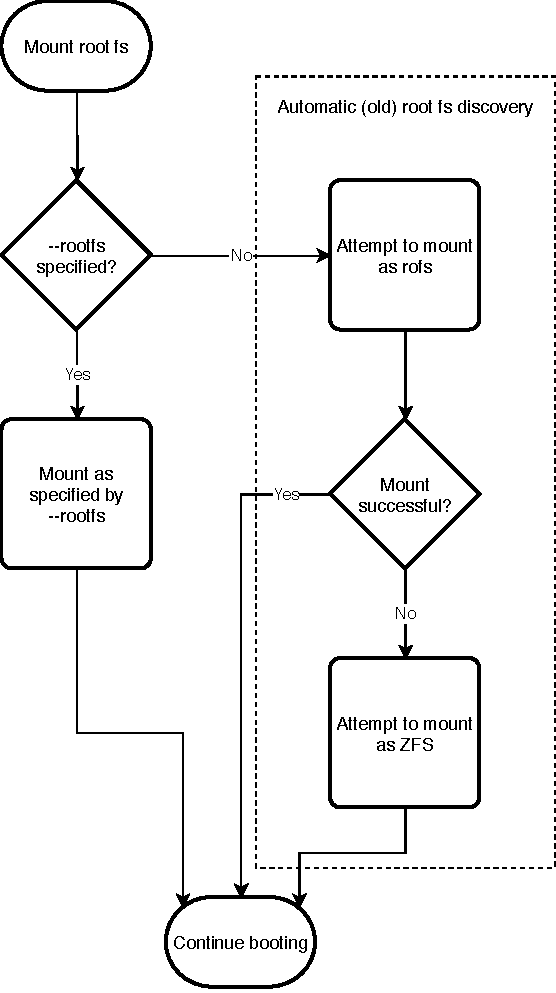
\includegraphics{rootfs}
    \caption{Η διαδικασία προσάρτησης του \en{root file system}.}
    \label{fig:rootfs}
\end{figure}

Τέλος, όσον αφορά καθεαυτό το \viofs{}, η χρήση του ως \en{root file system}
δεν ενείχε κάποια αξιοσημείωτη πρόκληση: εάν επιλέγονταν μέσω του
\texttt{\en{-{}-rootfs}}, γινόταν προσάρτηση του από την πρώτη \viofs{} συσκευή
(στο \osv{}, σε αντίθεση με το \en{linux}, αυτές εκτίθενται στο \en{devfs},
αριθμημένες σειριακά αντί να αναγνωρίζονται από το \viofs{} \en{tag} τους).
Προκειμένου να συμπληρωθεί αυτόματα με τα κατάλληλα περιεχόμενα για την εκάστοτε
εφαρμογή ένας κατάλογος στον \host{} (ο οποίος στη συνέχεια θα χρησιμοποιηθεί
ως το \viofs{} \en{shared directory}) είναι διαθέσιμες οι παράμετροι
\texttt{\en{export}} και \texttt{\en{export\_dir}} του \en{scripts/build}.

\chapter{Αξιολόγηση}

Για την αξιολόγηση του νέου συστήματος αρχείων στο \osv{}, διεξάγαμε δοκιμές
συγκρίνοντας με τα υπόλοιπα διαθέσιμα συστήματα αρχείων αλλά και το
\viofs{} στο \linux{}, όπου η σύγκριση είχε νόημα. Οι δοκιμές περιλαμβάνουν
τρία σενάρια, όπως αναλύονται στη συνέχεια: ένα συνθετικό μετροπρόγραμμα
(\en{synthetic benchmark} ή \en{microbenchmark}), μια δοκιμή χρόνου εκκίνησης
και τέλος μία πραγματική εφαρμογή (\en{application benchmark}).

\section{Μεθοδολογία}
Όλες οι δοκιμές πραγματοποιήθηκαν σε προσωπικό υπολογιστή με τα στοιχεία που
αναφέρονται στον πίνακα \ref{tab:host-specs}, ενώ ο πίνακας
\ref{tab:guest-specs} περιλαμβάνει τις προδιαγραφές των \osv{} και \linux{}
\en{guests}. Ως προς τη διεξαγωγή τους πρέπει να αναφερθούν τα εξής:
\begin{itemize}
    \item Για την εκτέλεση όλων των δοκιμών χρησιμοποιήθηκε ένα προσωρινό
          σύστημα αρχείων (\emph{\en{tmpfs}}) % ref https://www.kernel.org/doc/html/v5.8/filesystems/tmpfs.html
          στον \host{}, τόσο για τις εικόνες του \osv{} όσο και για τους
          κοινόχρηστους καταλόγους στην περίπτωση των \viofs{} και \en{NFS}.
          Αυτό έγινε ώστε να μην επηρεάζονται οι επιδόσεις από τη συσκευή
          αποθήκευσης του \host{}.
    \item Η δυναμική προσαρμογή της συχνότητας της \en{CPU} ήταν
          απενεργοποιημένη, χρησιμοποιώντας τον \emph{\en{``performance'' CPU
          scaling governor}} % ref https://www.kernel.org/doc/html/v5.8/admin-guide/pm/cpufreq.html
          στον \host{}.
    \item Η διεργασία του \qemu{} ήταν απομονωμένη από τις υπόλοιπες
          (\en{virtiofsd, perf, vegeta}) ως προς τις \en{CPUs} στις οποίες
          εκτελούνταν (\emph{\en{CPU pinning}}). % ref https://man7.org/linux/man-pages/man2/sched_setaffinity.2.html
          Συγκεκριμένα, στο \qemu{} αφιερώνονταν επεξεργαστικοί πυρήνες
          ισάριθμοι με το πλήθος των \en{CPUs} του \guest{}, ενώ οι υπόλοιπες
          προαναφερόμενες διεργασίες δεσμεύονταν στους υπόλοιπους διαθέσιμους.
          Αυτό έγινε με σκοπό την ελαχιστοποίηση των παρεμβολών που θα μπορούσαν
          να επηρεάσουν τις επιδόσεις.
    \item Για τη μέτρηση της χρησιμοποιούμενης επεξεργαστικής ισχύος (\en{CPU
          usage}) επελέγη το \emph{\en{perf}}. % TODO: cite https://perf.wiki.kernel.org/index.php/Main_Page
          Συγκεκριμένα, χρησιμοποιήθηκε η εντολή \texttt{\en{perf stat}}, με το
          \en{``task-clock'' perf event}. Η μέτρηση έγινε για τη διεργασία του
          \qemu{}, το \en{virtiofsd}, το \en{vhost kernel thread} και τα \en{NFS
          kernel threads} (για το καθένα όπου ήταν εφαρμόσιμο):
    \item Όλες οι δοκιμές επαναλήφθηκαν \emph{10 φορές}, από τις οποίες στη
          συνέχεια παρουσιάζονται η μέση τιμή \en{mean} και η τυπική απόκλιση
          \en{standard deviation}. Στην περίπτωση του \osv{} κάθε επανάληψη ήταν
          μία εκ νέου εκκίνηση της εικονικής μηχανής, ενώ στο \linux{} όλες οι
          επαναλήψεις έγιναν στην ίδια εκτέλεση της εικονικής μηχανής.
    \item Το \en{virtiofsd} εκτελούνταν με το \en{cache mode} απενεργοποιημένο
          (\texttt{\en{cache=none}}) και ένα \en{thread}
          (\texttt{\en{--thread-pool-size=1}}). Το δεύτερο επελέγη διότι
          οδηγούσε σε ελαφρώς πιο συνεπείς μετρήσεις, χωρίς όμως να παρατηρείται
          καλύτερη επίδοση όπως είχε αναφερθεί σε συζήτηση στη \en{mailing list}
          του \viofs{}%
          \footnote{\en{\url{https://www.redhat.com/archives/virtio-fs/2020-September/msg00068.html}}}.
    \item Για την εκτέλεση του \osv{} έγινε χρήση του βοηθητικού \en{script}
          (\en{scripts/run.py}) που παρέχει, το οποίο τροποποιήθηκε για την
          διεξαγωγή των δοκιμών, ώστε να ενορχηστρώνει την εκτέλεση όλων των
          υπόλοιπων εργαλείων (\en{virtiofsd, perf, vegeta}). Ως προς τη
          δικτύωση της εικονικής μηχανής, χρησιμοποιήθηκε το \emph{\en{tap
          backend}} % ref https://www.qemu.org/docs/master/system/invocation.html#hxtool-5
          του \qemu{} με το \emph{\en{vhost}} ενεργοποιημένο, ενώ στο \en{VM}
          δινόταν στατική διεύθυνση \en{IP}.
    \item Ως \en{NFS server} χρησιμοποιήθηκε η αντίστοιχη υλοποίηση του \linux{}
          στον \host{}. Όλες οι δοκιμές έγιναν με την έκδοση 3 του \en{NFS},
          καθώς η έκδοση 4 δεν ήταν λειτουργική από την πλευρά του \osv{} και
          με \en{readahead} στον \en{NFS client (libnfs)} ίσο με 2 \en{MiB} (όσο
          και το αντίστοιχο μέγεθος στην υλοποίηση μας του \en{virtio-fs DAX}).
\end{itemize}

\begin{table}
    \centering
    \begin{tabular}{ |c|c| }
        \hline
        Επεξεργαστής & \en{Intel Core i7-6700 @3.4GHz} \\
        \hline
        Μνήμη & 2\(\times\)8 \en{GiB @2666MHz} \\
        \hline
        \en{Swap} & Όχι \\
        \hline
        \en{Linux kernel} & \en{5.8.13-arch1-1} \\
        \hline
        \qemu{} & \en{5.1.50 @ c37a890d12e57a3d28c3c7ff50ba6b877f6fc2cc} \\
        % TODO: cite https://gitlab.com/virtio-fs/qemu/-/tree/c37a890d12e57a3d28c3c7ff50ba6b877f6fc2cc
        \hline
    \end{tabular}
    \caption{Προδιαγραφές του \host{} όπου διεξήχθησαν οι δοκιμές.}
    \label{tab:host-specs}
\end{table}

\begin{table}
    \centering
    \begin{tabular}{ |c|c| }
        \hline
        \en{CPUs} & 4 \\
        \hline
        Μνήμη & 4 \en{GiB} \\
        \hline
        \en{DAX window} & 4 \en{GiB} \\
        \hline
        \osv{} & \en{5372a230ce0abf0dc72e92ec1116208145e595c5} \\
        % TODO: cite https://github.com/cloudius-systems/osv/tree/5372a230ce0abf0dc72e92ec1116208145e595c5
        \hline
        \en{Linux kernel} & \en{5.8.0-rc4-33261-gfaa931f16f27} \\
        % TODO: cite https://gitlab.com/virtio-fs/linux/-/tree/faa931f16f27d37a1b688d6129cf70b801a81506
        \hline
    \end{tabular}
    \caption{Προδιαγραφές των \en{guests}.}
    \label{tab:guest-specs}
\end{table}

\section{\en{Microbenchmark}}
\subsection{Περιγραφή}
Για τη μέτρηση των επιδόσεων του συστήματος αρχείων χρησιμοποιήσαμε το
\en{flexible I/O tester (fio)} % TODO: cite https://github.com/axboe/fio
στην έκδοση 3.23. Προκειμένου να εκτελεστεί στο \osv{} χρειάστηκαν μόνο δύο
τροποποιήσεις%
\footnote{Όλες οι αλλαγές βρίσκονται στο ``\en{osv}'' \en{branch} του \en{git
repository \url{https://github.com/foxeng/fio}}.}
και τα κατάλληλα ορίσματα στο \en{configure script} του \en{fio} ώστε να
απενεργοποιηθούν χαρακτηριστικά που δεν παρέχονται από το \osv{}. Σημειώνουμε
ότι το ίδιο ακριβώς εκτελέσιμο (με τα παραπάνω απενεργοποιημένα) χρησιμοποιήθηκε
και στο \linux{}, εκτός από το \osv{}.

Στη σύγκριση περιλαμβάνονται τα \en{ZFS, rofs, ramfs}, \viofs{} (με και χωρίς
\en{DAX window}, με \en{ramfs root file system}) και \en{NFS} στο
\osv{}, το \viofs{} (με και χωρίς \en{DAX window}, με \en{ext4 root file
system}) στο \linux{}, καθώς και το \en{tmpfs} στον \host{}, το οποίο
συμπεριλάβαμε για πληρότητα, ως σημείο αναφοράς (\en{baseline}). Συγκεκριμένα
για τη διαδικασία έχουμε:
\begin{itemize}
    \item Σε όλες τις περιπτώσεις εκτός του \en{ramfs}, τα αρχεία ελέγχου
          (\en{test files}) του \en{fio} έχουν παραχθεί εκ των προτέρων από το
          ίδιο και έχουν τοποθετηθεί στην εκάστοτε τοποθεσία (εικονικό δίσκο ή
          κοινόχρηστο κατάλογο). Αυτό γίνεται παρότι το \en{fio} μπορεί να τα
          παράξει δυναμικά κατά το χρόνο εκτέλεσης, διότι κάποια από τα
          συστήματα αρχείων είναι \en{read-only}. Επειδή το \en{ramfs} είναι
          περιορισμένο ως προς το μέγεθος μεμονωμένων αρχείων στο \en{image}
          του, στην περίπτωση του τα αρχεία παράγονται κατά το χρόνο εκτέλεσης.
    \item Εξετάζονται δύο περιπτώσεις ως προς τα αρχεία ελέγχου:
          \begin{itemize}
              \item Ένα μεγάλο αρχείο (1 \en{GiB}).
              \item Πολλαπλά (10) μικρότερα αρχεία (80-100 \en{MiB}).
                    Σημειώνουμε ότι τα αρχεία σε όλες τις δοκιμές είναι
                    πανομοιότυπα (το αντίστοιχο αρχείο έχει το ίδιο μέγεθος
                    πάντα).
          \end{itemize}
          Και στις δύο περιπτώσεις το συνολικό μέγεθος των αρχείων δεν ξεπερνά
          το 1 \en{GiB}. Αυτό εν μέρει γίνεται διότι το μέγεθος αυτό είναι
          περιορισμένο από τη μνήμη του \guest{} για τα \en{rofs} και \en{ramfs}
          και το μέγεθος του \en{DAX window} για το \viofs{} με \en{DAX}.
    \item Εξετάζονται δύο περιπτώσεις ως προς το πρότυπο (\en{pattern})
          ανάγνωσης των αρχείων: σειριακό (\texttt{\en{rw=read}}) και τυχαίο
          (\texttt{\en{rw=randread}}). % ref https://github.com/foxeng/osv/tree/virtiofs-tests/modules/fio/tests
    \item Σε όλες τις περιπτώσεις υπάρχει μόνο \emph{ένα \en{thread}} ανάγνωσης
          (\texttt{\en{numjobs=1}}).
    \item Στο \linux{}, για την αυτοματοποίηση των δοκιμών βασιστήκαμε στο
          σχετικό βοήθημα του \en{Vivek Goyal}. % TODO: cite https://github.com/rhvgoyal/virtiofs-tests
          Αξίζει να σημειωθεί ότι το συγκεκριμένο ακυρώνει τις \en{page, inode}
          και \en{dentry caches} χρησιμοποιώντας το \en{sysctl} \\
          (\en{/proc/sys/vm/drop\_caches}) % ref https://www.kernel.org/doc/html/latest/admin-guide/sysctl/vm.html
          πριν από κάθε εκτέλεση του \en{fio}.
    \item Στην περίπτωση του \linux{} (\guest{} και \host{}) δεν έγινε μέτρηση
          του \en{CPU usage} γιατί μία τέτοια σύγκριση κρίθηκε ότι δεν έχει
          αξία, δεδομένου του διαφορετικού χαρακτήρα του από το \osv{}
          (λειτουργικό γενικού σκοπού από τη μία και \en{unikernel} από την
          άλλη).
\end{itemize}

\subsection{Αποτελέσματα}

\begin{figure}
    \begin{minipage}[c][\textheight]{\textwidth}
        \begin{subfigure}[c][0.5\textheight]{\textwidth}
            \caption{\en{Throughput}}
            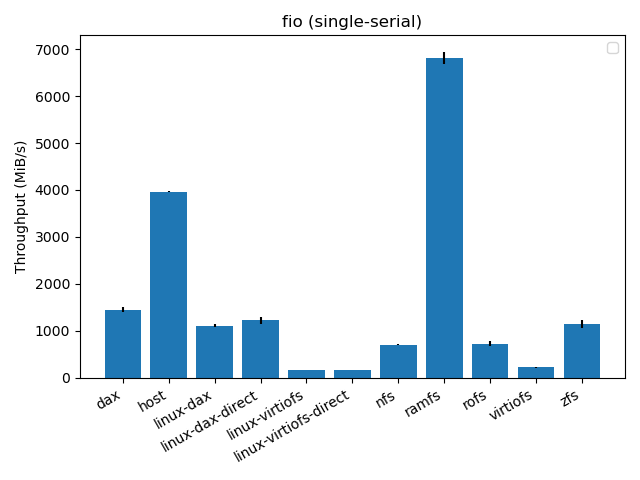
\includegraphics[width=\textwidth]{fio-single-serial-tput}
            \label{fig:fio-single-serial-tput}
        \end{subfigure}
        \begin{subfigure}[c][0.5\textheight]{\textwidth}
            \caption{\en{CPU usage}}
            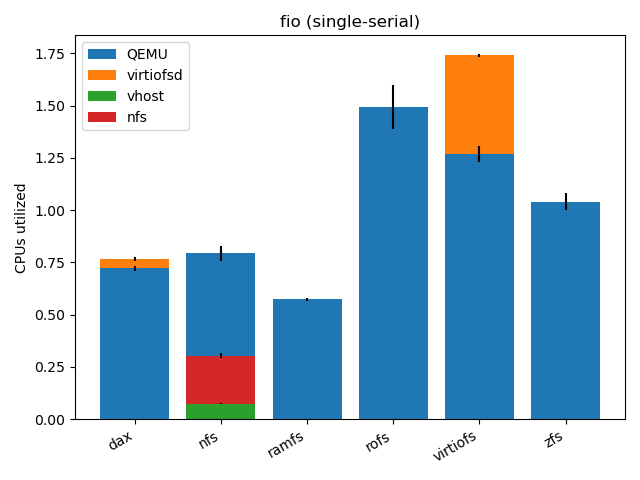
\includegraphics[width=\textwidth]{fio-single-serial-cpu}
            \label{fig:fio-single-serial-cpu}
        \end{subfigure}
        \caption{\en{fio}, ένα αρχείο, σειριακή ανάγνωση}
        \label{fig:fio-single-serial}
    \end{minipage}
\end{figure}

\begin{figure}
    \begin{minipage}[c][\textheight]{\textwidth}
        \begin{subfigure}[c][0.5\textheight]{\textwidth}
            \caption{\en{Throughput}}
            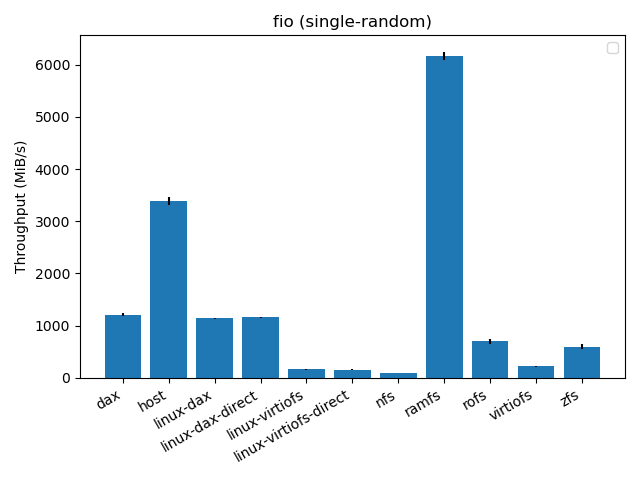
\includegraphics[width=\textwidth]{fio-single-random-tput}
            \label{fig:fio-single-random-tput}
        \end{subfigure}
        \begin{subfigure}[c][0.5\textheight]{\textwidth}
            \caption{\en{CPU usage}}
            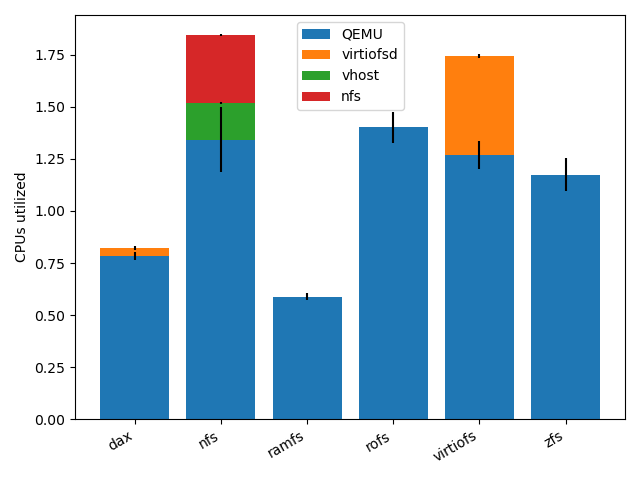
\includegraphics[width=\textwidth]{fio-single-random-cpu}
            \label{fig:fio-single-random-cpu}
        \end{subfigure}
        \caption{\en{fio}, ένα αρχείο, τυχαία ανάγνωση}
        \label{fig:fio-single-random}
    \end{minipage}
\end{figure}

\begin{figure}
    \begin{minipage}[c][\textheight]{\textwidth}
        \begin{subfigure}[c][0.5\textheight]{\textwidth}
            \caption{\en{Throughput}}
            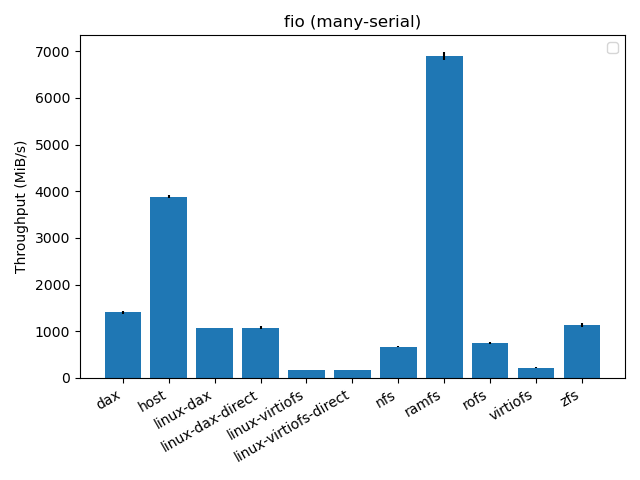
\includegraphics[width=\textwidth]{fio-many-serial-tput}
            \label{fig:fio-many-serial-tput}
        \end{subfigure}
        \begin{subfigure}[c][0.5\textheight]{\textwidth}
            \caption{\en{CPU usage}}
            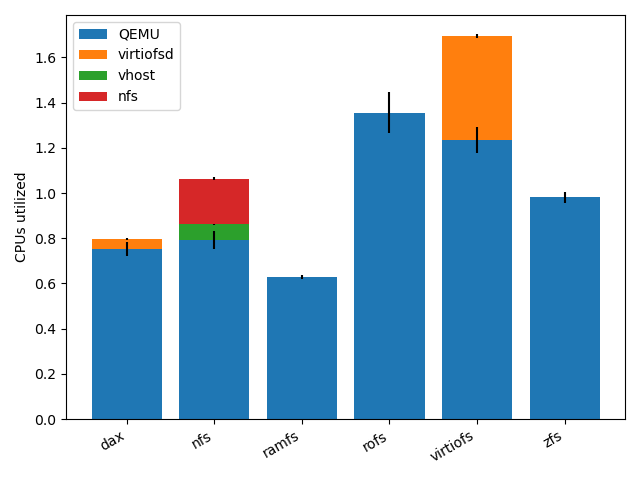
\includegraphics[width=\textwidth]{fio-many-serial-cpu}
            \label{fig:fio-many-serial-cpu}
        \end{subfigure}
        \caption{\en{fio}, πολλαπλά αρχεία, σειριακή ανάγνωση}
        \label{fig:fio-many-serial}
    \end{minipage}
\end{figure}

\begin{figure}
    \begin{minipage}[c][\textheight]{\textwidth}
        \begin{subfigure}[c][0.5\textheight]{\textwidth}
            \caption{\en{Throughput}}
            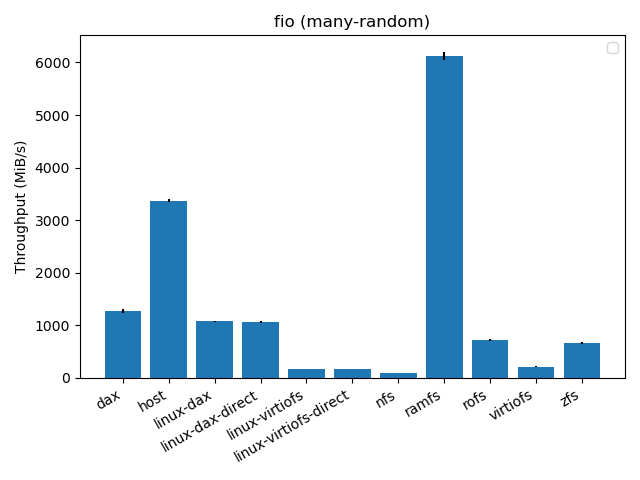
\includegraphics[width=\textwidth]{fio-many-random-tput}
            \label{fig:fio-many-random-tput}
        \end{subfigure}
        \begin{subfigure}[c][0.5\textheight]{\textwidth}
            \caption{\en{CPU usage}}
            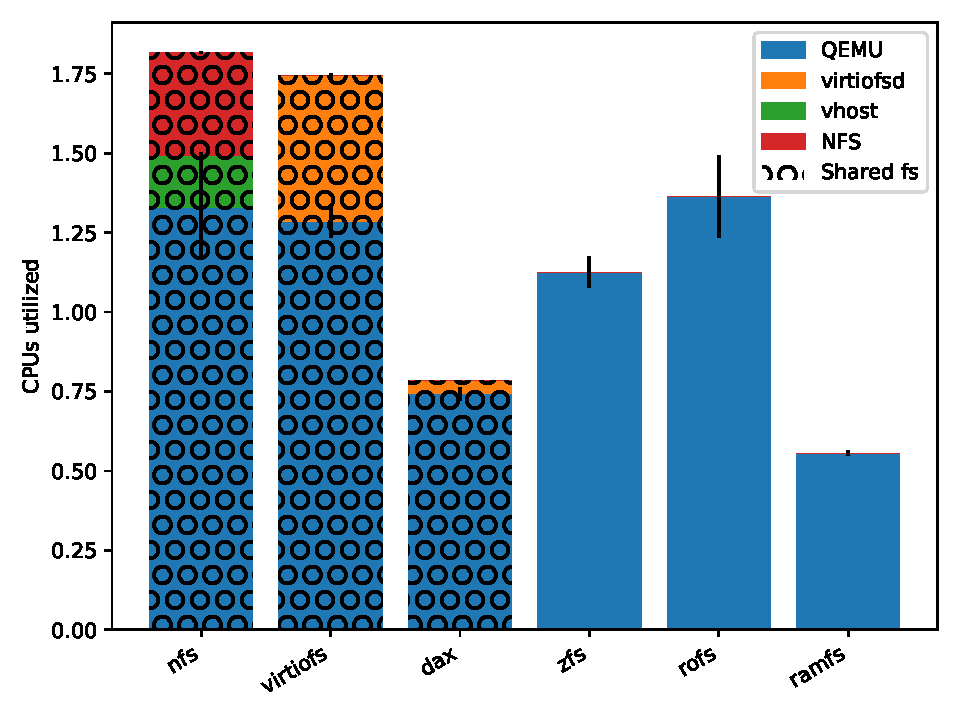
\includegraphics[width=\textwidth]{fio-many-random-cpu}
            \label{fig:fio-many-random-cpu}
        \end{subfigure}
        \caption{\en{fio}, πολλαπλά αρχεία, τυχαία ανάγνωση}
        \label{fig:fio-many-random}
    \end{minipage}
\end{figure}

% tst   OSv    Linux
%  s-s: 220  - 170  (virtio-fs)
%       1450 - 1108 (DAX)
%       707         (NFS)
%  s-r: 217  - 163  (virtio-fs)
%       1212 - 1142 (DAX)
%       85          (NFS)
%  m-s: 219  - 166  (virtio-fs)
%       1402 - 1071 (DAX)
%       668         (NFS)
%  m-r: 215  - 166  (virtio-fs)
%       1269 - 1081 (DAX)
%       85          (NFS)
% mean: 217  - 166  (virtio-fs)
%       1333 - 1100 (DAX)
%       386         (NFS)

Όπως βλέπουμε στα σχήματα \ref{fig:fio-single-serial} έως
\ref{fig:fio-many-random}, το υψηλότερο \en{throughput} επιτυγχάνεται από το
\en{ramfs} στο \osv{}, υψηλότερο και από αυτό του \en{tmpfs} στον \host{}. Αυτό
συμβαίνει διότι, με τα δεδομένα στη μνήμη το \en{virtualization overhead}
ελαχιστοποιείται, ενώ ταυτόχρονα η απλοποιημένη υλοποίηση του συστήματος αρχείων
και η έλλειψη \en{mode switches} λόγω κλήσεων συστήματος στο \osv{} φαίνεται ότι
κάνουν τη διαφορά. Το \viofs{} με \en{DAX} προσφέρει τις αμέσως καλύτερες
επιδόσεις στο \osv{}, σε όλες τις περιπτώσεις, και παράλληλα έχει τη μικρότερη
επιβάρυνση σε όρους επεξεργαστικής ισχύος, και πάλι μετά το \en{ramfs}.

Εστιάζοντας στο \viofs{} και συγκρίνοντας ανάμεσα σε \osv{} και \linux{},
διακρίνουμε συνεπή συμπεριφορά σε όλες τις περιπτώσεις: σε αμφότερα τα
λειτουργικά το \en{DAX window} υπερτερεί του \viofs{} χωρίς αυτό με μεγάλη
διαφορά (\(> 6 \times\) \en{throughput}), ενώ στο \osv{} βλέπουμε \(20 - 30 \%\)
καλύτερες επιδόσεις από ότι στο \linux{}. Το δεύτερο είναι αναμενόμενο, αφενός
λόγω της απλούστερης υλοποίησης στο \osv{}, που υποστηρίζει πολύ λιγότερες
λειτουργίες και αφετέρου λόγω των συγκριτικών πλεονεκτημάτων ενός
\en{unikernel}.

Ιδιαίτερη μνεία οφείλουμε στη σύγκριση ανάμεσα σε \viofs{} και \en{NFS}, τα μόνα
κοινόχρηστα συστήματα αρχείων στο \osv{}. Εδώ το \viofs{} με \en{DAX window}
έχει το προβάδισμα στις επιδόσεις, με το \en{NFS} να ακολουθεί και το \viofs{}
χωρίς \en{DAX} να βρίσκεται τελευταίο, στις δοκιμές με σειριακή ανάγνωση.
Όπως φαίνεται και στον πίνακα \ref{tab:fio-virtiofs-nfs}, στις δοκιμές τυχαίας
ανάγνωσης τα αποτελέσματα διαφοροποιούνται, με το \en{NFS} να έχει το χειρότερο
\en{throughput} (και μεγαλύτερο \en{CPU usage}), έχοντας επηρεαστεί σαφώς
περισσότερο σε σχέση με το \viofs{} από την αλλαγή στο \en{access pattern}.

\begin{table}
    \centering
    \begin{tabular}{ |c|c|c|c| }
        \hline
        \en{pattern} & \viofs{} & \en{NFS} & \viofs{} \en{DAX} \\
        \hline
        σειριακό & 1,0 & 3,1 & 6,5 \\
        τυχαίο & 1,0 & 0,4 & 5,7 \\
        \hline
    \end{tabular}
    \caption{Κανονικοποιημένο \en{fio throughput} \viofs{} και \en{NFS} στο
        \osv{}.}
    \label{tab:fio-virtiofs-nfs}
\end{table}

\section{Χρόνος εκκίνησης}
\subsection{Περιγραφή}
Προκειμένου να αξιολογήσουμε τον χρόνο εκκίνησης στο \viofs{} επιλέξαμε μία
εφαρμογή από αυτές που έχουν ήδη μεταφερθεί στο \osv{} ως παραδείγματα. % TODO: cite https://github.com/cloudius-systems/osv-apps
Συγκεκριμένα, επελέγη το \en{spring-boot-example}, μια απλή \en{web} εφαρμογή
από το % TODO: cite https://github.com/in28minutes/spring-boot-examples
χτισμένη με το \en{spring boot framework}, % ref https://spring.io/projects/spring-boot
στην έκδοση του 2.3.4.%
\footnote{Όλες οι αλλαγές που έγιναν για τις δοκιμές μας βρίσκονται στο
``\en{virtiofs-tests}'' \en{branch} του \en{git repository
\url{https://github.com/foxeng/osv-apps}}.}
Ως \en{Java runtime} επιλέξαμε και πάλι από την ίδια
συλλογή εφαρμογών το \en{openjdk8-zulu-full}. % ref https://github.com/cloudius-systems/osv-apps/tree/master/openjdk8-zulu-full
Η επιλογή της συγκεκριμένης εφαρμογής έγινε καθώς θεωρήθηκε αντιπροσωπευτική,
ως \en{stateless web app}, εφαρμογής που θα γινόταν \en{deploy} ως
\en{unikernel}, σε ένα πλαίσιο \en{cloud}.

Στις δοκιμές συμμετείχαν όλα τα συστήματα αρχείων του \osv{} τα οποία μπορούν να
χρησιμοποιηθούν ως \en{root file systems: ZFS, rofs, ramfs} και \viofs{}.

Η διαδικασία περιελάμβανε την εκκίνηση του \osv{} με το εκάστοτε σύστημα αρχείων
να χρησιμοποιείται ως \en{root file system}. Αυτό αφηνόταν να τρέξει για ένα
εύλογο χρονικό διάστημα κάποιων δευτερολέπτων, μέσα στο οποίο ολοκληρωνόταν η
πλήρης αρχικοποίηση της εφαρμογής και στη συνέχεια τερματιζόταν από το μηχανισμό
(\en{script}) ενορχήστρωσης των δοκιμών, τερματίζοντας τη διεργασία του \qemu{}.

\subsection{Αποτελέσματα}
Στο σχήμα \ref{fig:startup-app} απεικονίζεται μία ανάλυση του συνολικού χρόνου
εκκίνησης ως εξής:
\begin{description}
    \item[\en{OSv boot}] είναι ο χρόνος εκκίνησης (\en{boot}) του συστήματος του
                         \osv{}, δηλαδή του μέρους που είναι ανεξάρτητο της
                         εκάστοτε εφαρμογής.
    \item[\en{Root fs mount}] είναι ο χρόνος προσάρτησης (\en{mount}) του
                              \en{root file system} και της αλλαγής της
                              ``ρίζας'' (\en{/}) του εικονικού συστήματος
                              αρχείων σε αυτό (\en{pivot}). Επισημαίνεται ότι
                              αυτό είναι ένα στάδιο του προηγούμενου, αλλά εν
                              προκειμένω έχει αφαιρεθεί από εκείνο και
                              παρουσιάζεται χωριστά.
    \item[\en{Application}] είναι o χρόνος αρχικοποίησης της ίδιας της
                            εφαρμογής, όπως καταγράφεται από αυτήν.
\end{description}

\begin{figure}
    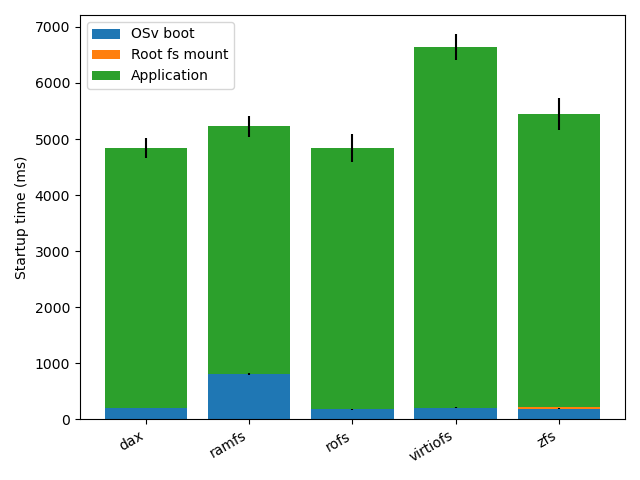
\includegraphics[width=\textwidth]{startup-app}
    \caption{\en{Spring boot example}, χρόνοι εκκίνησης}
    \label{fig:startup-app}
\end{figure}

% fs        total time
% ZFS       5452
% rofs      4838
% ramfs     5226
% virtio-fs 6642
% DAX       4844

Όπως βλέπουμε καλύτερα στον πίνακα \ref{tab:startup-total}, με όρους συνολικού
χρόνου εκκίνησης, το \viofs{} \emph{χωρίς} \en{DAX window} υστερεί έναντι των
υπολοίπων, ενώ το \viofs{} \emph{με} \en{DAX window} έχει την καλύτερη επίδοση,
μαζί με το \en{rofs} (τα \en{ramfs} και \en{ZFS} είναι ελαφρώς πιο αργά).

\begin{table}
    \centering
    \begin{tabular}{ |c|c|c|c|c| }
        \hline
        \en{ZFS} & \en{rofs} & \en{ramfs} & \viofs{} & \viofs{} \en{DAX} \\
        \hline
        1,13 & 1,00 & 1,08 & 1,37 & 1,00 \\
        \hline
    \end{tabular}
    \caption{Κανονικοποιημένος συνολικός χρόνος εκκίνησης
        \en{spring-boot-example} στο \osv{}.}
    \label{tab:startup-total}
\end{table}

Όσον αφορά τον χρόνο προσάρτησης (\en{mount time}), για όλα τα συστήματα αρχείων
είναι πρακτικά αμελητέος (\(<2\%\) του \osv{} \en{boot time}), \emph{εκτός από
το \en{ZFS}}. Στην περίπτωση του τελευταίου, ο χρόνος προσάρτησης αποτελεί
περίπου το \(14\%\) του χρόνου εκκίνησης του συστήματος, κάτι αναμενόμενο
δεδομένης της πολυπλοκότητας του συγκεκριμένου συστήματος αρχείων, η οποία
μεταφράζεται σε μία σαφώς πιο μακρά διαδικασία αρχικοποίησης.

Τέλος, αξίζει να αναφερθούμε στον αισθητά αυξημένο χρόνο εκκίνησης του \osv{}
στην περίπτωση του \en{ramfs}. Αυτή η διαφοροποίηση δικαιολογείται εάν
αναλογιστούμε ότι στην περίπτωση του \en{ramfs}, το \en{root file system}
\emph{ταυτίζεται} με το \en{boot file system} (σε ορολογία \osv{}, το αντίστοιχο
\en{initramfs} στο \linux{}). Αυτό είναι μέρος του \en{ELF object} που περιέχει
το \en{kernel}, το οποίο φορτώνεται και αποσυμπιέζεται κατά τα πρώιμα στάδια του
\en{boot}, % TODO: cite https://github.com/cloudius-systems/osv/wiki/OSv-early-boot-(MBR)
σε μια διαδικασία με χαμηλό \en{throughput}, λόγω του περιορισμένου αρχικού
περιβάλλοντος. Έτσι, όταν στην περίπτωση του \en{ramfs}, το εν λόγω \en{ELF
object} είναι έως και μία τάξη μεγέθους μεγαλύτερο από τα υπόλοιπα, αυτό
είναι υπαίτιο για την αύξηση του χρόνου εκκίνησης. Βέβαια, εν προκειμένω έχουμε
κάνει κατάχρηση του \en{ramfs}, το οποίο δεν είναι προορισμένο για τόσο μεγάλα
\en{images}.

\section{\en{Application benchmark}}
\subsection{Περιγραφή}
Για να αξιολογήσουμε το \viofs{} με όρους μιας ολοκληρωμένης, πραγματικής
εφαρμογής επιλέξαμε και πάλι από το πεδίο των \en{stateless} εφαρμογών σε
πλαίσιο \en{cloud} το σενάριο ενός στατικού \en{web} εξυπηρετητή (\en{server}).
Συγκεκριμένα, χρησιμοποιήσαμε τον \en{nginx} % TODO: cite http://nginx.org/
(στην έκδοση του 1.19.2), έναν από τους πλέον δημοφιλείς \en{web servers}
ελεύθερου λογισμικού, ο οποίος είναι επίσης διαθέσιμος στη συλλογή εφαρμογών του
\osv{}.%
\footnote{Όλες οι αλλαγές που έγιναν για τις δοκιμές μας βρίσκονται στο
``\en{virtiofs-tests}'' \en{branch} του \en{git repository
\url{https://github.com/foxeng/osv-apps}}.}

Στις δοκιμές συμμετείχαν τα όλα τα συστήματα αρχείων του \osv{} (στην περίπτωση
του \viofs{}, ως \en{root file system} χρησιμοποιήθηκε το \en{ramfs})
\emph{εκτός από το \en{NFS}}, με το οποίο το σενάριο μας αποτύγχανε.
Συγκεκριμένα, κατά την εξυπηρέτηση του πρώτου αιτήματος (\en{request}) από τον
\en{server}, μετά την αποστολή λίγων αρχικών δεδομένων της απάντησης
(\en{response}), η διαδικασία σταματούσε και ο \guest{} φαινόταν ``παγωμένος''.
Αυτό διαπιστώθηκε ότι δεν οφείλονταν στον \en{nginx}, καθώς την ίδια ακριβώς
συμπεριφορά επιδείκνυε το σύστημα με τον \en{lighttpd} (επίσης περιλαμβάνεται
στη συλλογή του ``\en{osv-apps}'') στη θέση του. Περαιτέρω διερεύνηση απαιτείται
για να εντοπιστεί και πιθανώς να διορθωθεί η αιτία, η οποία από την εμπειρία μας
φαίνεται να μοιάζει με κάποιου είδους ``αδιέξοδο'' που πιθανώς να εντοπίζεται
στην υλοποίηση του \en{NFS} ή της στοίβας δικτύωσης του \osv{}.

Τα αρχεία τα οποία εξέθετε ο \en{web server} ήταν συνολικά 10, με μέγεθος που
κυμαίνονταν από περίπου 500 \en{KiB} μέχρι και 12 \en{MiB}. Το μέγεθος κάθε
αντίστοιχου αρχείου ήταν σταθερό σε όλες τις δοκιμές.

Για την διεξαγωγή των δοκιμών, που είχαν τη μορφή δοκιμών φορτίου \en{HTTP}
(\en{HTTP load tests}), από τη μεριά του πελάτη (\en{HTTP client})
χρησιμοποιήσαμε το \en{vegeta}, % TODO: cite https://github.com/tsenart/vegeta
ένα δημοφιλές εργαλείο γι' αυτό το σκοπό, στην έκδοση του 12.8.3. Η διαδικασία
(αυτοματοποιημένη από το \en{script} ενορχήστρωσης) είχε ως εξής:
\begin{enumerate}
    \item Αρχικά εκκινούνταν ο \osv{} \guest{}, στον οποίο δίνονταν ένα
          δευτερόλεπτο περιθώριο προκειμένου να ολοκληρωθεί η αρχικοποίηση του
          \en{nginx server}).
    \item Στον \host{} εκκινούσε το \en{vegeta}, ρυθμισμένο να παράγει \en{HTTP
          1.1 GET requests} για όλα τα αρχεία του \en{server}, με το μέγιστο
          δυνατό ρυθμό, χρησιμοποιώντας 20 ``εργάτες'' και έως 4 \en{CPUs}, με
          την επαναχρησιμοποίηση (\en{keepalive}) των συνδέσεων \en{TCP}
          ενεργοποιημένη.
    \item Μετά από δέκα δευτερόλεπτα, το \en{vegeta} ολοκλήρωνε το έργο του και
          τερματιζόταν, οπότε και ο αυτοματισμός τερμάτιζε τον \guest{} μέσω
          της διεργασίας του \qemu{}.
\end{enumerate}

\subsection{Αποτελέσματα}

\begin{figure}
    \begin{minipage}[c][\textheight]{\textwidth}
        \begin{subfigure}[c][0.5\textheight]{\textwidth}
            \caption{\en{Requests} ανά δευτερόλεπτο}
            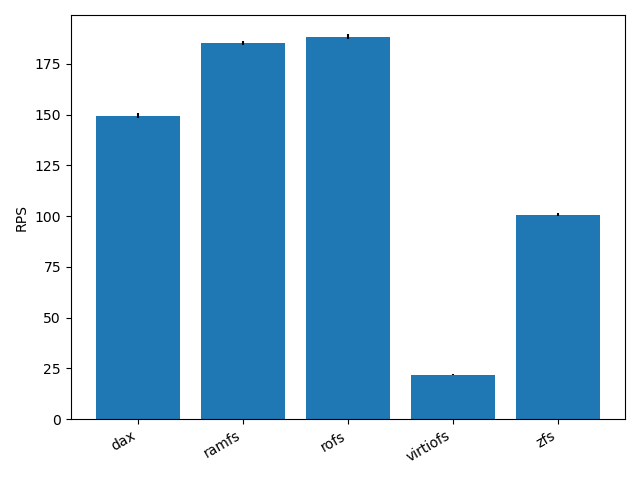
\includegraphics[width=\textwidth]{nginx-rps}
            \label{fig:nginx-rps}
        \end{subfigure}
        \begin{subfigure}[c][0.5\textheight]{\textwidth}
            \caption{\en{CPU usage}}
            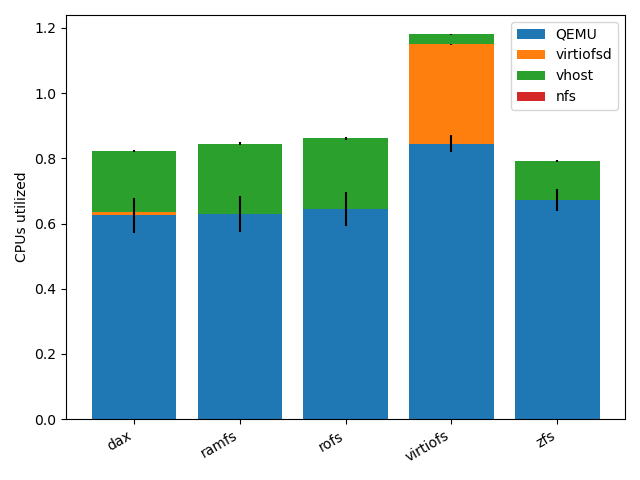
\includegraphics[width=\textwidth]{nginx-cpu}
            \label{fig:nginx-cpu}
        \end{subfigure}
        \caption{\en{nginx HTTP load test}}
        \label{fig:nginx}
    \end{minipage}
\end{figure}

% fs        rps
% ZFS       100
% rofs      188
% ramfs     185
% virtio-fs 150
% DAX       22

Όπως βλέπουμε στο σχήμα \ref{fig:nginx-rps}, το \viofs{} με \en{DAX window}
προσφέρει \en{throughput} (σε όρους εξυπηρετούμενων αιτημάτων ανά δευτερόλεπτο)
που υπολείπεται αυτού των \en{rofs} και \en{ramfs} (τα οποία προηγούνται) κατά
\(\sim 20\%\). Δεδομένου ότι το \en{CPU usage} είναι οριακά χαμηλότερο από των
άλλων δύο, αυτή η διαφορά χρήζει περαιτέρω μελλοντικής διερεύνησης (μέσω
\en{profiling}), με εστίαση στην υλοποίηση του \viofs{} με \en{DAX read
datapath} στο \osv{}, ως κύριο ύποπτο.

Όπως είναι αναμενόμενο σε αυτό το σενάριο χρήσης, το \viofs{} χωρίς \en{DAX}
υστερεί με διαφορά έναντι όλων των υπόλοιπων συστημάτων αρχείων. Αυτό διότι
είναι το μόνο που δεν χρησιμοποιεί οποιασδήποτε μορφής κρυφή μνήμη (\en{cache})
και κάθε λειτουργία ανάγνωσης συνεπάγεται έξοδο και επεξεργασία στον \host{}
(όπως φαίνεται και από το υψηλό \en{CPU usage}), ενώ αυτές οι λειτουργίες είναι
πολύ συχνές, πολλαπλασιάζοντας τις συνέπειες αυτού του \en{overhead}.

\chapter{Συμπεράσματα και επεκτάσεις}


\appendix
\selectlanguage{english}

\chapter{FUSE copyright notice}
\label{app:copyright}

\noindent
Copyright (C) 2001-2007 Miklos Szeredi. All rights reserved.

\vspace{2ex}
\noindent
Redistribution and use in source and binary forms, with or without modification,
are permitted provided that the following conditions are met:
\begin{enumerate}
	\item Redistributions of source code must retain the above copyright notice,
		  this list of conditions and the following disclaimer.
	\item Redistributions in binary form must reproduce the above copyright
		  notice, this list of conditions and the following disclaimer in the
		  documentation and/or other materials provided with the distribution.
\end{enumerate}

\noindent
THIS SOFTWARE IS PROVIDED BY AUTHOR AND CONTRIBUTORS ``AS IS'' AND
ANY EXPRESS OR IMPLIED WARRANTIES, INCLUDING, BUT NOT LIMITED TO, THE
IMPLIED WARRANTIES OF MERCHANTABILITY AND FITNESS FOR A PARTICULAR PURPOSE
ARE DISCLAIMED.  IN NO EVENT SHALL AUTHOR OR CONTRIBUTORS BE LIABLE
FOR ANY DIRECT, INDIRECT, INCIDENTAL, SPECIAL, EXEMPLARY, OR CONSEQUENTIAL
DAMAGES (INCLUDING, BUT NOT LIMITED TO, PROCUREMENT OF SUBSTITUTE GOODS
OR SERVICES; LOSS OF USE, DATA, OR PROFITS; OR BUSINESS INTERRUPTION)
HOWEVER CAUSED AND ON ANY THEORY OF LIABILITY, WHETHER IN CONTRACT, STRICT
LIABILITY, OR TORT (INCLUDING NEGLIGENCE OR OTHERWISE) ARISING IN ANY WAY
OUT OF THE USE OF THIS SOFTWARE, EVEN IF ADVISED OF THE POSSIBILITY OF
SUCH DAMAGE.

\selectlanguage{greek}


\bibliographystyle{babplain}
\bibliography{main}

\end{document}
